% =====================================================================
%  Data Compatibility as a Bottleneck in Cross-Country Earthquake
%  Damage Modelling: Nepal--T\"urkiye Transfer and a Japan Contrast Case
%  Camilla Andreozzi
%  Major-revision draft addressing IJDRR peer-review feedback
% =====================================================================

\documentclass[11pt,a4paper]{article}

% ---------- Packages ----------
\usepackage[utf8]{inputenc}
\usepackage[T1]{fontenc}
\usepackage{lmodern}
\usepackage{amsmath, amssymb, amsthm}
\usepackage{graphicx}
\usepackage{booktabs}
\usepackage{tabularx}
\usepackage{longtable}
\usepackage{multirow}
\usepackage{caption}
\usepackage{subcaption}
\usepackage{geometry}
\usepackage{hyperref}
\usepackage{xcolor}
\usepackage{enumitem}
\usepackage{microtype}
\usepackage{setspace}
\usepackage{natbib}
\usepackage{authblk}
\usepackage{tcolorbox}
\usepackage{array}
\usepackage{ragged2e}
\geometry{margin=2.5cm}
\hypersetup{colorlinks=true, linkcolor=black, citecolor=blue, urlcolor=blue}

% ---------- Custom commands ----------
\newcommand{\Y}{\ensuremath{Y}}
\newcommand{\X}{\ensuremath{\mathcal{X}}}
\newcommand{\Tk}{T\"urkiye}

\newtcolorbox{kbox}[1][]{colback=gray!5, colframe=gray!50,
  title=#1, fonttitle=\bfseries, sharp corners, boxrule=0.4pt}

% ---------- Title ----------
\title{\textbf{Data compatibility as a bottleneck in cross-country earthquake damage modelling}}

\author[1]{Camilla Andreozzi}
\affil[1]{\small Independent author. Correspondence: andreozzicamilla@gmail.com}

\date{\today}

\begin{document}

\maketitle


\begin{abstract}
\noindent
Disaster risk reduction (DRR) increasingly depends on post-disaster damage models that can be reused across countries to support inspection prioritisation, reconstruction, risk financing and vulnerability assessment. Whether such reuse is possible depends less on classifier choice than on whether national post-event datasets describe buildings, hazards and damage in comparable ways. We test this directly using asset-level inventories from Nepal ($n=762{,}094$), T\"urkiye ($n=242$) and Japan ($n=140{,}208$), with Nepal and T\"urkiye forming a survey-based transfer pair and Japan included as a reduced-specification stress test on a distance-only feature space. Within country, Random Forest reaches binary AUC $0.864$ on Nepal and around $0.70$ on T\"urkiye; cross-country transfer on the harmonised Nepal--T\"urkiye core falls below the no-skill benchmark in both directions (AUC $0.434$ and $0.450$), and the three-country distance-only stress test produces below-chance Japan transfer (T\"urkiye$\rightarrow$Japan $0.365$, Nepal$\rightarrow$Japan $0.428$). A controlled simulation, run within an explicit scenario grid, indicates that for discrimination metrics the compatibility regime explains substantially more performance variance than the choice of classifier. The implication for DRR is that reusable damage modelling requires post-event data infrastructure --- not better algorithms alone; we therefore propose a minimum standardised asset-level variable core for post-event surveys and post-disaster data governance, intended for inclusion in national reconnaissance protocols and Sendai Monitor-compatible reporting.
\end{abstract}
\newpage

\tableofcontents
\newpage

% =====================================================================
\section{Introduction}
\label{sec:intro}
% =====================================================================

Earthquake damage assessment at the asset level is central to disaster risk reduction (DRR), post-disaster response and recovery planning. A rapid understanding of which buildings are likely to be damaged, severely damaged or destroyed informs inspection prioritisation, emergency-resource allocation, reconstruction planning, exposure and vulnerability databases used for risk financing, and the design of future risk-reduction interventions. This problem has historically been addressed through engineering vulnerability and fragility functions, which relate structural damage to one or more hazard-intensity measures under predefined assumptions about building classes and response behaviour \citep{yepes2016vulnerability, rossetto2014empirical, erdik2017earthquake}. Their use in cross-country analysis depends on whether buildings, vulnerability classes and exposure attributes are defined consistently enough to make damage estimates comparable across datasets and regions \citep{silva2022buildingclass, yepes2023exposure}. Over the last decade, machine-learning techniques have entered the same problem space as a flexible complement: rather than imposing a fixed functional relationship between hazard and damage, they learn directly from labelled observations and incorporate a wider range of predictors simultaneously \citep{xie2020review, mangalathu2020classifying, breiman2001randomforests}. Their flexibility increases the demands placed on the underlying data, because a learner can only extract from the data what the data contain, and only carry across contexts what the contexts have in common. This problem is also a policy problem. The Sendai Framework for Disaster Risk Reduction \citep{unisdr2015sendai} explicitly identifies the production and sharing of comparable hazard, exposure and loss data as part of Priority 1 ("understanding disaster risk"), and the Sendai Monitor targets A–D depend on loss accounting that is consistent across countries. Climate-resilient infrastructure commitments under the Paris Agreement \citep{unfccc2015paris} create the same demand from the adaptation side. Both frameworks therefore presume the kind of harmonised asset-level damage information that this paper takes as its empirical object.

The same machine-learning toolkit is now embedded in a growing disaster-risk modelling and decision-support literature that goes beyond classifying damage. Recent work uses tree ensembles to estimate post-earthquake reconstruction grants from seismic vulnerability features \citep{rosso2026grants}, explainable AI to translate urban ground-subsidence risk predictions into inspection and maintenance decisions \citep{lee2026subsidence}, and boosted models such as LightGBM to improve wildfire burned-area prediction from early fire-perimeter geometry \citep{kim2026wildfireifd, ke2017lightgbm}. Although these studies span different hazards and decision settings, they share a common dependency on well-defined, interoperable hazard, exposure and impact data. The contribution of the present paper is upstream of those pipelines: rather than proposing another classifier, it stress-tests the feasibility of cross-country machine-learning frameworks under the compatibility constraints that current post-disaster datasets present, and treats the resulting modelling exercise as a foundational data-infrastructure step for the DRR-oriented catastrophe-modelling literature it serves.

The pressing question for that wider literature is not which model classifies damage best within a single event --- that has been extensively studied in country-specific contexts \citep{ghimire2022nepal, hariri2025turkiye} --- but whether widely available post-disaster datasets actually permit cross-country generalisation. The intersection of jointly observable predictors across countries collapses quickly as geographic scope expands because the underlying datasets are produced under different collection protocols, with different variable definitions and units, consistent with broader calls for systematic standardisation of cross-border seismic risk assessment \citep{rosti2021aedes, fakhruddin2022riskinformed, babic2025crossborder}. Whatever flexibility a machine-learning model offers, the signal it can extract is limited by the harmonised feature space --- the set of variables jointly observable across countries.

The novelty of this paper lies in combining, on the same three-country empirical base, five elements that have so far been pursued separately: (i) a measurement-compatibility audit that distinguishes \emph{direct}, \emph{convertible}, \emph{coarse-proxy} and \emph{not-compatible} variables across Nepal, T\"urkiye and Japan; (ii) a Nepal--T\"urkiye cross-country transfer experiment on a small harmonised feature core; (iii) a reduced-specification Japan stress test under a deliberately minimal, distance-only specification ($F_0$); (iv) a controlled simulation that separates the contribution of compatibility regime from the contribution of model class to performance variance; and (v) a minimum standardised asset-level variable core proposed as a concrete deliverable for post-event survey instruments and Sendai Monitor-compatible reporting (Table~\ref{tab:min-core}). The aim of the paper is therefore not another classifier benchmark; it is to identify a data-governance bottleneck that limits reusable post-disaster evidence across countries, and to propose a minimum asset-level variable core for future survey protocols. We address four research questions:

\begin{enumerate}[label=(RQ\arabic*),leftmargin=*]
  \item Which asset-level earthquake damage variables are directly
        compatible, convertible, available only as coarse proxies, or
        unavailable across Nepal, T\"urkiye and Japan?
  \item How much predictive performance is lost when moving from
        country-specific Nepal and T\"urkiye feature sets to a
        harmonised Nepal--T\"urkiye core?
  \item Does poor cross-country transfer appear more consistent with
        data incompatibility than with classifier choice? (Japan enters
        this question as a reduced-specification stress test on a
        distance-only feature space, $F_0$.)
  \item What minimum post-event asset-level variable core would improve
        future DRR modelling and survey interoperability?
\end{enumerate}

The datasets have different roles. Nepal supplies a very large post-Gorkha 2015 inventory with ordinal damage grades and rich building typology, but only a coarse hazard proxy \citep{ghimire2022nepal}. T\"urkiye supplies a much smaller 2023 engineering reconnaissance sample with detailed structural variables and stronger shaking information \citep{hariri2025turkiye}. These two survey-based datasets form the main transfer experiment. Japan adds a 2024 Noto Peninsula remote-sensing damage inventory \citep{vescovo2025noto}. It is not treated as a third symmetric training country; instead, it is brought into the modelling step under a deliberately reduced specification ($F_0$), in which an asset-level distance to the Noto epicentre is used as a minimal proxy feature shared with Nepal and T\"urkiye, while country-specific hazard overlays (tsunami, fire, slope failure) are excluded from any pooled or transfer fit. This makes Japan a stress test of cross-country generalisation under harsher harmonisation, rather than a third symmetric modelling country.

The paper proceeds in three steps. First, it audits the compatibility of the source variables. Second, it benchmarks within-country models, Nepal--T\"urkiye transfer on a small harmonised core, and the three-country Japan stress test on $F_0$. Third, it uses ablation and simulation to assess whether the observed limits are more consistent with data compatibility or with classifier choice. The main contribution to DRR is therefore not another classifier; it is an empirical argument, backed by a concrete proposal (Table~\ref{tab:min-core}), that transferable earthquake damage modelling requires standardised post-event asset-level data. Section~\ref{sec:litreview} reviews the relevant literature. Section~\ref{sec:data} describes the datasets and compatibility matrix. Section~\ref{sec:methods} introduces the methodology. Section~\ref{sec:results} reports the empirical and simulation results. Section~\ref{sec:discussion} discusses implications for transferability and post-disaster data infrastructure, and Section~\ref{sec:conclusion} concludes.

% =====================================================================
\section{Literature review}
\label{sec:litreview}
% =====================================================================

The literature relevant to this paper sits at the intersection of three strands of work that have grown closer to each other over the last decade. 
The first strand concerns the expanding use of machine learning in post-disaster damage assessment and disaster-risk
modelling. In the earthquake-damage literature, supervised learning has been widely used to classify damage in event- or country-specific settings. Comprehensive reviews emphasise that, once a flexible non-linear classifier is in place, data quality, feature engineering and labelling decisions tend to dominate the choice of algorithm \citep{xie2020review}; benchmark comparisons consistently find that random forests and gradient-boosted ensembles emerge as competitive baselines on tabular post-earthquake datasets \citep{mangalathu2020classifying, breiman2001randomforests, ke2017lightgbm}. Within particular events, \citet{ghimire2022nepal} apply supervised learning to the regional-scale 2015 Gorkha building damage inventory in Nepal, exploiting broad typological and geometric predictors, while \citet{hariri2025turkiye} provide data driven insights from the 2023 T\"urkiye-sequence reconnaissance using a more engineering-rich predictor set; the present study draws data from both of those sources and partially adopts the latter's modelling framework. More recently, transferability has become a first-class evaluation question in image-based damage assessment, with \citet{lin2022transfer} examining transfer learning for seismic building damage assessment from imagery, \citet{zheng2024transferable} investigating transferable damage assessment via domain-adaptive change detection, and \citet{chen2025bright} introducing the BRIGHT benchmark for robust transfer across disasters and geographies.

The same machine-learning toolkit is also increasingly embedded in broader disaster-risk modelling and decision-support pipelines that go beyond classifying damage. Closest in spirit to the present empirical experiment, \citet{ghimire2024host} test machine-learning damage classifiers trained in one country (e.g.\ Nepal, Haiti, Italy, Serbia) and scored on another, and report that out-of-region accuracy is bounded by data quality and contextual similarity rather than by classifier sophistication. On the opposite end of the data-availability spectrum, \citet{patten2024datadriven} train multi-impact damage models on roughly 370{,}000 buildings across 26 earthquakes in 61 countries and reach AUC near 0.93 on a 2023 T\"urkiye holdout, illustrating that scale and harmonisation can together overcome much of the cross-country gap that smaller, heterogeneous corpora cannot.\citet{rosso2026grants} use ensemble methods to predict post-earthquake reconstruction grants for masonry buildings from seismic vulnerability features, demonstrating that machine learning can support the financial and reconstruction-decision side of earthquake recovery directly from asset-level structural descriptors. \citet{lee2026subsidence} propose an explainable-AI framework that converts urban subsidence-risk predictions into practical maintenance and investigation decisions, while \citet{kim2026wildfireifd} combine initial fractal dimension with LightGBM to improve wildfire burned-area prediction. Across these applications, the cumulative message is that algorithmic flexibility within a single event or decision setting is no longer the main constraint. What remains underdeveloped is the portability of such models across countries, especially when they rely on tabular asset-level data whose definitions, units and collection protocols differ. The present paper therefore sits upstream of these modelling pipelines and asks empirically whether the data foundations on which they depend can support cross-country deployment at all.

The second strand concerns the disaster-risk-reduction literature on data availability, comparability and interoperability. The closest precedent to the question addressed here is the standardisation of building classification, exposure data and post-event survey instruments. \citet{silva2022buildingclass} introduce a building classification system designed for multi-hazard risk assessment, the GED4ALL framework, explicitly motivated by the need for interoperability between datasets; \citet{yepes2023exposure} present the global building exposure model used by the Global Earthquake Model, which standardises exposure descriptors across countries; and \citet{yepes2016vulnerability} document the GEM physical vulnerability database, which compiles vulnerability functions in standardised form to enable comparison across studies. The same impulse drives the harmonisation of national post-event survey forms with international taxonomies. \citet{rosti2021aedes} convert information collected through Italy's AeDES form, and centralised in the Da.D.O.\ platform, into GEM-compatible attributes and EMS-98 building classes via a score-based methodology, illustrating that significant scientific value can be extracted from existing
post-event surveys provided the mapping to recognised standards is made explicit.

At the same time, the literature also shows that post-earthquake damage datasets differ not only in which variables they contain but in how those variables are produced. \citet{stone2018omnidirectional} discuss the use of omnidirectional imagery for systematic earthquake damage data collection, \citet{adriano2021multimodal} emphasise the growing role of multimodal Earth-observation data in building damage mapping, and \citet{vescovo2025noto} document the construction of the 2024 Noto Peninsula damage inventory as a combination of multi-source remote sensing with crowd-sourced verification and independent checking. These are fundamentally different measurement regimes from engineering reconnaissance or administrative recovery surveys. Incompatibility across post-earthquake datasets is therefore not merely a missing-column problem but a measurement-regime problem: a building age recorded by an engineering team during physical inspection is not the same observable as a building footprint inferred from remote sensing, even when both are reduced to the same column name. Hybrid empirical-analytical approaches \citep{noh2015hybrid} combine the strengths of multiple data regimes precisely because no single regime is sufficient on its own. Existing taxonomies standardise how buildings, exposure descriptors and vulnerability classes are described before an event; the missing layer addressed here is the harmonisation of observed post-event damage inventories used to train and validate data-driven models.

The third strand sets these distinctions in the wider context of data-informed resilience. \citet{fakhruddin2022riskinformed} frame disaster and climate resilience as a risk-informed data problem in which actionable resilience requires data that are comparable, accessible and produced under shared standards, consistent with the FAIR data principles \citep{wilkinson2016fair} and with the monitoring requirements of the Sendai Framework for Disaster Risk Reduction. From this perspective, post-disaster damage data are not only inputs to predictive models but part of the evidence infrastructure through which disaster risk reduction is monitored, evaluated and translated into policy-relevant decisions. The same diagnosis appears outside the seismic-hazard literature: \citet{bressan2024assetlevel} show that asset-level climate physical-risk assessment is fundamentally constrained by the availability and standardisation of granular asset data, indicating that the harmonisation problem is a recognised cross-hazard issue rather than a peculiarity of post-earthquake datasets. Closer to the seismic-risk side, \citet{babic2025crossborder} propose a framework for harmonised cross-border assessment that integrates hazard, exposure and fragility models, reinforcing the argument that interoperability cannot be solved at the modelling layer alone. Bringing the strands together, the literature supports three propositions: machine learning has improved single-event damage prediction and is increasingly being deployed in catastrophe and recovery-decision pipelines; cross-country generalisation depends on the availability of compatible data structures and comparable measurement regimes; and risk-informed resilience requires interoperable data infrastructure rather than isolated country-specific datasets. The contribution of this paper fills that gap.
% =====================================================================
\section{Data}
\label{sec:data}
% =====================================================================

The three datasets used in this paper differ not only in country and earthquake context but in data-generating process, spatial scale and variable design. Each country is described below through a common five-part template — event and study context, data source and collection protocol, hazard representation, asset-level variables, and damage labels and limitations — and is then summarised, alongside the others, in an explicit compatibility matrix. Sample sizes, class balance and missingness are reported in a single comparable table at the end of the section so that the reader can see the asymmetries that the modelling experiments must contend with.

% ---------------------------------------------------------------
\subsection{T\"urkiye}
\label{sec:data-turkiye}

\paragraph{Event and study context.} The 6 February 2023 earthquake sequence consisted of a first main shock of $M_w = 7.81$ near Pazarc{\i}k followed by a major aftershock of $M_w = 6.7$ near Nurda\u{g}{\i}, a second large event of $M_w = 7.52$ near Elbistan, and a further $M_w = 6.3$ event affecting Hatay on 20 February. The sequence produced severe losses across a region containing a substantial share of the national building stock and economic output.

\paragraph{Data source and collection protocol.} The database was assembled from direct field observations of \textbf{242 reinforced-concrete buildings} surveyed as part of the ACI~133 reconnaissance effort \citep{hariri2025turkiye}. Each building was inspected by a small engineering team using visual inspection, plan sketching, measurement of major structural elements, photographic documentation and three-dimensional scanning. The dataset is therefore a structured post-disaster engineering survey, with the strengths and limits that such a regime implies.

\paragraph{Hazard representation.} Hazard variables were not measured at each building but estimated by combining strong-motion recordings from AFAD's Turkish Accelerometric Database with ground-motion modelling and spatial interpolation. The resulting hazard package includes PGA, PGV, spectral acceleration at multiple periods, Arias intensity, cumulative absolute velocity and distance-related variables.

\paragraph{Asset-level variables.} Building age, number of storeys, total height, floor area, column area at the critical floor, reinforced-concrete and masonry wall areas in two orthogonal directions, captive-column indicator, soft-storey indicator, several derived engineering indices and the site condition $V_{s30}$. Table~\ref{tab:turkiye-vars} summarises these variables.

\paragraph{Damage labels and limitations.} Both structural and non-structural damage labels are provided. For modelling we use the structural label simplified into ordinal categories. Because the observed damage reflects the outcome of an earthquake sequence rather than a single isolated loading episode, the labels should be understood as post-sequence observed damage states.

\begin{table}[!t]
\centering
\caption{Asset-side variables available in the T\"urkiye dataset.}
\label{tab:turkiye-vars}
\small
\begin{tabularx}{\linewidth}{l X}
\toprule
\textbf{Variable family} & \textbf{Variables} \\
\midrule
Identification / location & \texttt{id, latitude, longitude} \\
Basic geometry & \texttt{age, no\_stories, no\_stories\_above\_critical\_floor\_cf,
total\_height, floor\_area, total\_floor\_area\_above\_c\_f} \\
Vertical structural elements & \texttt{c\_f\_column\_area} \\
Wall-system descriptors &
\texttt{c\_f\_concrete\_wall\_area\_\{ns,ew\}},
\texttt{c\_f\_masonry\_wall\_area\_\{ns,ew\}},
\texttt{critical\_aac\_masonry\_wall\_area\_\{ns,ew\}} \\
Directional summaries &
\texttt{c\_f\_concrete\_wall\_area\_\{max,min\}},
\texttt{c\_f\_masonry\_wall\_area\_\{max,min\}} \\
Irregularity indicators & \texttt{captive\_columns\_presence, soft\_story} \\
Engineering indices &
\texttt{column\_index\_percent, wall\_index\_\{ns,ew\}\_percent,
min\_wi\_percent, priority\_index\_percent, cd, wd} \\
Site condition & \texttt{v\_s30} \\
\bottomrule
\end{tabularx}
\end{table}

% ---------------------------------------------------------------
\subsection{Nepal}
\label{sec:data-nepal}

\paragraph{Event and study context.} The 25 April 2015 Gorkha earthquake ($M_w = 7.8$) affected a large share of the country, caused close to nine thousand deaths, displaced millions and generated losses of national significance.

\paragraph{Data source and collection protocol.} The dataset was assembled during the post-earthquake reconstruction period by the National Planning Commission together with Kathmandu Living Labs and the Central Bureau of Statistics \citep{ghimire2022nepal}. Data collection took place between January and May 2016, and the cleaned working dataset contains \textbf{762{,}094 building-level observations}.

\paragraph{Hazard representation.} The principal hazard variable is \texttt{district\_distance\_to\_earthquakecenter} (in miles in the source file). The earthquake is therefore represented through a derived spatial proxy rather than through directly measured or modelled local intensity. This is the dataset's main hazard limitation and is examined explicitly as a compatibility-regime sensitivity in Section~\ref{sec:methods}.

\paragraph{Asset-level variables.} Building age, number of floors, plinth area, building height (per-storey or total height depending on source release; Section~\ref{sec:data-cleaning} documents how this is handled in our pipeline), foundation type, roof type, ground-floor type, building position, and a set of binary indicators for primary superstructure material (mud-mortar stone, cement-mortar brick, timber, bamboo, RC engineered, RC non-engineered and others). Table~\ref{tab:nepal-vars} summarises these.

\paragraph{Damage labels and limitations.} Damage labels follow the EMS-98 framework \citep{grunthal1998ems98} with five ordinal grades from negligible damage (DG1) to destruction (DG5). Labels were assigned during the reconstruction period rather than during emergency response, the hazard variable is only a proxy, and some variables contain placeholder-style extreme values that require careful cleaning (Section~\ref{sec:data-cleaning}).

\begin{table}[!t]
\centering
\caption{Main asset-level variables in the Nepal dataset.}
\label{tab:nepal-vars}
\small
\begin{tabularx}{\linewidth}{l X}
\toprule
\textbf{Group} & \textbf{Variables} \\
\midrule
Administrative & \texttt{vdcmun\_id, ward\_id} \\
Basic geometry & \texttt{count\_floors\_pre\_eq, age\_building,
plinth\_area\_sq\_ft, per-height\_ft\_pre\_eq} \\
Site / terrain & \texttt{land\_surface\_condition} \\
Foundation & \texttt{foundation\_type} \\
Roof & \texttt{roof\_type} \\
Ground floor & \texttt{ground\_floor\_type} \\
Building position & \texttt{position} \\
Superstructure (binary) &
\texttt{has\_superstructure\_\{adobe\_mud, mud\_mortar\_stone,
stone\_flag, cement\_mortar\_stone, mud\_mortar\_brick,
cement\_mortar\_brick, timber, bamboo, rc\_non\_engineered,
rc\_engineered, other\}} \\
Hazard proxy & \texttt{district\_distance\_to\_earthquakecenter(mi)} \\
\bottomrule
\end{tabularx}
\end{table}

% ---------------------------------------------------------------
\subsection{Japan}
\label{sec:data-japan}

\paragraph{Event and study context.} Japan is included to show what happens when the measurement regime changes. The 2024 Noto Peninsula earthquake of 1 January 2024 was an $M_w = 7.5$ event associated with severe shaking and multi-hazard impacts, including tsunami, landslides, ground deformation and fire \citep{vescovo2025noto,
usgs2024noto}.

\paragraph{Data source and collection protocol.} The Noto dataset is a georeferenced building-damage inventory compiled from multi-source remote sensing, opt-in crowd-sourced verification and independent checking \citep{vescovo2025noto}. It contains pre-event building footprints for \textbf{140{,}208 structures}. This is not the same type of source as Nepal or T\"urkiye. Those datasets are survey-based building inventories; the Japan dataset is primarily a footprint-based remote-sensing inventory.

\paragraph{Hazard and asset information.} The dataset includes USGS Modified Mercalli Intensity and binary overlays for tsunami, fire and slope-failure exposure. It is strong on spatial footprint geometry, but it does not provide building age, number of storeys, total height or structural system in a form that is directly comparable with Nepal and T\"urkiye. Table~\ref{tab:japan-vars} summarises the principal Japan variables.

\paragraph{Role in this paper.} Japan is used as a reduced-specification stress test rather than as a third symmetric training domain. The question is twofold: what remains of the modelling feature space when a remote-sensing post-event inventory is added, and whether the most reductive physical predictor that all three countries can plausibly observe --- distance to the source --- still carries common signal across them. To make this question precise, we deliberately exclude the country-specific hazard overlays (tsunami, fire, slope failure) from any shared model: these are recorded in Japan only, and including them in a pooled model would let Japan's classifier exploit information that has no analogue in Nepal or T\"urkiye. We instead compute an asset-level distance from each Noto building footprint to the 2024 epicentre ($137.272^\circ$E, $37.498^\circ$N; USGS event \texttt{us6000m0xl}) using \texttt{sf::st\_point\_on\_surface} after geometry repair, in the WGS-84 frame. This recovers a single continuous predictor for Japan that is dimensionally and conceptually compatible with Nepal's district-level distance-to-epicentre and T\"urkiye's building-specific epicentral distance, which together define the cross-country distance-only feature space $F_0$ used in Section~\ref{sec:results}. The Japan within-country baseline retains the GSI overlays only for an upper-bound comparison, never for the pooled or transfer experiments. This framing avoids making a rhetorical three-country modelling claim while preserving the main value of Japan for this paper: it lets the cross-country argument about data infrastructure be tested under a more reductive but jointly observable specification.

\begin{table}[!t]
\centering
\caption{Main asset and contextual variables in the Japan dataset.}
\label{tab:japan-vars}
\small
\begin{tabularx}{\linewidth}{l X}
\toprule
\textbf{Group} & \textbf{Variables} \\
\midrule
Identifier & \texttt{s\_fid} \\
Source / provenance & \texttt{source, conf} \\
Administrative context & \texttt{municipality} \\
Geometry & \texttt{geom} (MULTIPOLYGON, EPSG:4326) \\
Damage label & \texttt{damage\_val}, \texttt{damage\_2} \\
Hazard overlays & \texttt{GSI\_fire, GSI\_tsunami, GSI\_slope\_failure} \\
Macroseismic intensity & \texttt{USGS\_MMI} \\
\bottomrule
\end{tabularx}
\end{table}

% ---------------------------------------------------------------
\subsection{Compatibility matrix and harmonisation justifications}
\label{sec:data-compat-matrix}

The compatibility matrix in Table~\ref{tab:compat-matrix} is the central descriptive product of this section. For each conceptual variable family, we record whether the variable is directly available, convertible (a unit change or simple recoding), available only as a coarse proxy, or not compatible in each country.

\begin{table}[!t]
\centering
\caption{Cross-country variable compatibility matrix. ``Direct''
denotes operationally identical variables; ``Convertible''
denotes one-to-one mappings via unit or coding change;
``Coarse proxy'' denotes a related but conceptually weaker
variable; ``Not comp.'' denotes no usable analogue.
Justifications for the ``Convertible'' and ``Coarse proxy'' cells
are listed below the table.}
\label{tab:compat-matrix}
\small
\begin{tabularx}{\linewidth}{X l l l}
\toprule
\textbf{Conceptual variable} & \textbf{Nepal} & \textbf{T\"urkiye} & \textbf{Japan} \\
\midrule
Building age (years)                & Direct        & Direct       & Not comp. \\
Number of storeys                   & Direct        & Direct       & Not comp. \\
Floor area / footprint area         & Convertible (ft$^2 \to$ m$^2$) & Direct & Geometry only \\
Total building height               & Convertible (ft $\to$ m) & Direct & Not comp. \\
Structural-system descriptor (typology) & Categorical (rich) & RC only & Not comp. \\
Wall-system descriptors             & Coarse proxy & Direct (rich) & Not comp. \\
Site condition ($V_{s30}$ or analogue) & Not comp. & Direct & Not comp. \\
PGA / PGV / SA at $T_1$             & Not comp. & Direct & Not comp. \\
Macroseismic intensity (MMI)        & Not comp. & Not comp. & Direct \\
Distance-to-source (km)             & Convertible (mi $\to$ km) & Direct & Coarse proxy \\
Tsunami / fire / slope overlays     & Not comp. & Not comp. & Direct (binary) \\
Ordinal damage grade (5-class)      & Direct (EMS-98) & Convertible ($N/L/M/S/C$) & Not comp. \\
Binary damage label (severe / not)  & Convertible & Convertible & Direct \\
Geolocation                         & Admin polygon (vdc/ward) & Point (lat/lon) & Polygon (footprint) \\
\bottomrule
\end{tabularx}
\end{table}

\paragraph{Justifications for the convertible and coarse-proxy cells.} Floor area and total height are converted from imperial to SI units using fixed conversion factors ($1\,\text{ft}^2 = 0.0929\, \text{m}^2$, $1\,\text{ft} = 0.3048\,\text{m}$); the operational risk is that Nepal's plinth area refers to the building's plinth footprint while T\"urkiye's floor area refers to the typical floor, and the two are conceptually equivalent only for single-storey buildings or for buildings without vertical set-backs. Similarly, Nepal's \texttt{district\_distance\_to\_earthquakecenter} (mi) and T\"urkiye's \texttt{m7\_8\_repi} (km) are both distances from a mainshock epicentre, but the Nepal value is a district-level aggregate while the T\"urkiye value is the building-specific epicentral distance for the 7.8 mainshock; a one-to-one mapping therefore equates a coarse spatial aggregate with an asset-level measurement. Wall-system descriptors are listed as coarse-proxy for Nepal because the dataset only encodes the dominant superstructure material rather than directional wall areas; the T\"urkiye damage label is convertible to EMS-98-style ordinal classes via the standard correspondence $N{\mapsto}1, L{\mapsto}2, M{\mapsto}3, S{\mapsto}4, C{\mapsto}5$, but the original semantics are reinforced-concrete-specific and the mapping is operational rather than physical; and Japan's footprint geometry can be collapsed to a footprint area but is not directly equivalent to a building floor area. The negative cross-country transfer documented in Section~\ref{sec:results} is partly driven by precisely the conversions that this table catalogues. The matrix makes one fact explicit. The size of the jointly available predictor set shrinks rapidly as countries are added. For Nepal and T\"urkiye, a usable common ordinal damage target plus a small structural and hazard core can be assembled. For Nepal, T\"urkiye and Japan, the universally comparable feature space is too thin for a symmetric three-country asset-level transfer model. This is not an algorithmic failure; it is a data-availability and measurement-regime fact.

% ---------------------------------------------------------------
\subsection{Sample sizes, class balance and missingness}
\label{sec:data-samples}

Table~\ref{tab:samples} reports total sample size, ordinal five-class distribution, binary severe-versus-non-severe distribution and missingness for each dataset. The asymmetry between the three datasets is severe and is essential to the interpretation of every modelling result that follows: Nepal is three orders of magnitude larger than T\"urkiye, T\"urkiye's grade DG5 contains only six buildings (which makes the five-class T\"urkiye task structurally rare-class-limited), and Japan has no ordinal label at all.

\begin{table}[!t]
\centering
\caption{Sample size, class distribution and missingness for each country. Five-class column counts are after the harmonisation mapping; missingness is reported as the proportion of records with missing target before complete-case filtering. Severe-class proportion is reported on the binary target $\Y^{(2)}$. For Japan, the five-class target is unavailable by design rather than missing after filtering.}
\label{tab:samples}
\small
\begin{tabular}{l r r r r r r r r}
\toprule
& & \multicolumn{5}{c}{\textbf{Five-class counts}} & \textbf{Severe} & \textbf{Missingness} \\
\cmidrule(lr){3-7}
Country & $n$ & DG1 & DG2 & DG3 & DG4 & DG5 & prop.\ $\Y^{(2)}{=}1$ & $\Y^{(5)}$ / $\Y^{(2)}$ \\
\midrule
Nepal     & 762{,}094 & 78{,}815 & 87{,}257 & 136{,}412 & 183{,}844 & 275{,}766 & 0.603 & 0\% / 0\% \\
T\"urkiye & 242       & 19       & 42       & 24        & 151       & 6         & 0.649 & 0\% / 0\% \\
Japan     & 140{,}208 & ---      & ---      & ---       & ---       & ---       & 0.199 & n/a / 0\% \\
\bottomrule
\end{tabular}
\end{table}

% ---------------------------------------------------------------
\subsection{Cleaning rules and data preparation}
\label{sec:data-cleaning}

We document the cleaning rules explicitly so that the modelling pipeline can be reproduced and so that the operational implications of the harmonisation choices remain visible. For Nepal we drop placeholder records flagged with extreme values such as $999$ years for age or $99$ feet for per-height, convert \texttt{plinth\_area\_sq\_ft} from ft$^2$ to m$^2$ via the factor $0.0929$, convert \texttt{per-height\_ft\_pre\_eq} from ft to m via $0.3048$, and convert \texttt{district\_distance\_to\_earthquakecenter(mi)} from miles to km via $1.60934$. Where the source release is ambiguous on whether the height variable is per-storey or total, we treat it as a height-related continuous predictor and document the ambiguity; this affects the absolute interpretation of the \texttt{total\_height\_m} feature but not the modelling result, which depends on monotone within-country variation. For T\"urkiye we map the ordinal damage label $\{N,L,M,S,C\}$ to $\{1,2,3,4,5\}$ and otherwise preserve the source variables. For Japan we retain \texttt{damage\_2} as the binary target, drop obstructed-view and missing-or-inconsistent records, and use the building footprint geometry, USGS MMI and the GSI overlays. The binary target is constructed in all cases as $\Y^{(2)} = \mathbf{1}\{\Y^{(5)} \in \{4,5\}\}$. All cleaning rules and conversions are implemented in the harmonisation script of the supplementary material.

% =====================================================================
\section{Methods}
\label{sec:methods}
% =====================================================================

The empirical strategy proceeds in three linked steps. First, we audit the compatibility of the Nepal, T\"urkiye and Japan datasets and define the harmonised feature spaces that can be compared across settings. Second, we evaluate within-country performance, pooled Nepal--T\"urkiye learning, cross-country transfer, overlap ablation and robustness diagnostics. Third, we use a controlled simulation to isolate the contribution of the compatibility regime from the contribution of model choice. Two prediction tasks are defined where the data allow them: a five-class ordinal damage classification problem on the harmonised target $\Y^{(5)}$, and a binary severe-versus-non-severe classification problem on $\Y^{(2)}$. Nepal and T\"urkiye supply both targets and therefore form the main modelling experiment. Japan does not support the same ordinal task and is not used as a symmetric training domain.

\subsection{Compatibility audit and feature-set construction}
\label{subsec:methods-compatibility}

The modelling design starts from an explicit hierarchy of nested feature sets. We define $F_0$, the maximally reductive three-country specification, as $\{\texttt{hazard\_proxy\_distance\_km}\}$ alone, where this single predictor is best understood as a \emph{minimal proxy feature} rather than a fully harmonised hazard variable: each country contributes a different operational object (Nepal's district-level distance, T\"urkiye's building-specific epicentral distance, and Japan's footprint-level distance to the 2024 Noto epicentre, computed as described in Section~\ref{sec:data-japan}), and the transfer experiment derives much of its scientific value from showing that even this superficially common predictor is not physically transferable across the three contexts. $F_0$ is the only specification fitted on all three countries jointly; it explicitly excludes Japan-only hazard overlays so the pooled and transfer experiments do not silently exploit predictors with no analogue in Nepal or T\"urkiye. We define $F_1$, the minimal Nepal--T\"urkiye common core, as $\{\texttt{age}, \texttt{no\_stories}, \texttt{floor\_area\_m2}, \texttt{total\_height\_m}, \texttt{hazard\_proxy\_distance\_km}\}$, with the harmonisation rules described in Section~\ref{sec:data-cleaning}. A categorical indicator \texttt{country} is added in pooled models to capture systematic source differences. We then define $F_2$ as $F_1$ plus a single coarse structural-system descriptor obtained by collapsing Nepal's superstructure indicators and T\"urkiye's RC-only sample into a shared categorical encoding (\texttt{masonry\_low, masonry\_high, rc, timber\_bamboo, other}). $F_3$ is the country-specific full predictor set used as the upper-bound within-country benchmark for Nepal and T\"urkiye separately. $J_1$ is the Japan within-country reference set comprising footprint area, USGS MMI, the three GSI overlays and the asset-level distance to the Noto epicentre; it is reported only as a Japan-specific upper-bound and never used in pooled or transfer fits. Japan therefore enters the cross-country experiments only through $F_0$, and as a reduced-specification stress-test case rather than as a third symmetric transfer country.

\subsection{Modelling pipeline and transfer protocol}
\label{subsec:methods-empirical}

Four model classes are evaluated: logistic / multinomial regression, proportional-odds ordinal regression \citep{mccullagh1980regression}, Random Forest \citep{breiman2001randomforests} and a feed-forward neural network. Implementation uses R~4.x with packages \texttt{ranger} for Random Forest ($B = 300$ trees, default \texttt{mtry}, \texttt{min.node.size} $= 1$, \texttt{replace} $=$ \texttt{TRUE}), \texttt{nnet} for the neural network with one hidden layer of 8 units (\texttt{maxit} $=$ 200, \texttt{MaxNWts} $=$ 2000) and for multinomial regression via \texttt{nnet::multinom}, \texttt{MASS::polr} for proportional-odds regression and base \texttt{glm} for binary logistic regression. Rows with missing values in the selected outcome or harmonised predictors are removed on a complete-case basis within each task. For neural-network and logistic-regression models, categorical variables are one-hot encoded and continuous predictors are standardised using training-set statistics only.

Within-country benchmarks for Nepal and T\"urkiye on $F_3$ use five-fold stratified cross-validation (\texttt{rsample::vfold\_cv} with \texttt{strata} = target). The cross-country transfer experiments use the harmonised core $F_1$ and estimate the following configurations: train Nepal and test T\"urkiye; train T\"urkiye and test Nepal; and train pooled Nepal+T\"urkiye and test held-out within pooled, with and without the country indicator. Results are recorded in a single long dataframe with columns \texttt{(train\_domain, test\_domain, feature\_set, model, task, metric, value, split\_id, country\_indicator)}. Macro-F1 is reported because the five-class target is severely imbalanced and the operational interest is in the full grade ladder rather than only the modal class; binary AUC is reported because it is invariant to the decision threshold and to the binary base rate, which differ markedly between Nepal (0.603) and T\"urkiye (0.649).

The Japan stress-test design is layered on top of this: (i) a within-country Japan binary benchmark on $J_1$, fitted with five-fold stratified cross-validation and Random Forest plus binary logistic regression; (ii) within-country $F_0$ baselines for Nepal, T\"urkiye and Japan, again with five-fold stratified cross-validation; (iii) a pooled three-country $F_0$ Random Forest, fitted with and without a categorical country indicator under five-fold cross-validation stratified by country to ensure each fold contains all three countries; and (iv) a $3\times 3$ train-to-test transfer matrix on $F_0$, where each off-diagonal cell is a single train-on-A / test-on-B fit and each diagonal cell is the corresponding 80/20 within-country split (used only as a comparison anchor for the transfer cells). The pooled and transfer fits never see the GSI overlays; those are confined to the Japan within-country reference baseline. The same long-format result schema is used, with \texttt{feature\_set = "F0"} flagging the three-country experiments.

The overlap-ablation experiment takes $F_1$ and removes predictors in a pre-specified order to form $K_5 \supset K_4 \supset K_3 \supset K_2 \supset K_1$, with hazard distance retained until last because it is the predictor most likely to survive in poor data regimes. At each level, all model classes are re-fitted and evaluated. Performance is recorded through standard discrimination and calibration metrics: accuracy, balanced accuracy and macro-F1 for the five-class task, and accuracy, sensitivity, specificity, precision, F1, AUC and Brier score for the binary task. Results are reported as the cross-validated mean and standard deviation across the five folds.

Because random pooled splits can inflate within-country performance through spatial leakage, for instance when buildings from the same Nepalese district appear in both train and test folds, we report an additional grouped cross-validation diagnostic for the Nepal binary Random Forest in which folds are grouped by \texttt{vdcmun\_id}. The random-split results remain the headline numbers because they match the evaluation protocol used in much of the single-event earthquake-damage literature, but the grouped diagnostic is reported in Section~\ref{sec:results} as a robustness check on geographic generalisation. Supplementary diagnostics also compute country-stratified partial-dependence curves, simple country-specific logistic marginal effects on the harmonised $F_1$ predictors, held-out confusion matrices and calibration diagnostics. These diagnostics are used to evaluate whether negative transfer is accompanied by predictor-direction changes, class-wise failure modes and probability-calibration issues.

\subsection{Controlled simulation}
\label{subsec:methods-simulation}

The empirical experiments cannot, on their own, separate the contribution of the harmonisation regime from the contribution of the chosen classifier: each Nepal--T\"urkiye or three-country fit changes the data and the model simultaneously, and the very small T\"urkiye sample inflates the variance of any single estimate. The controlled simulation is designed to isolate exactly this confound. It deliberately does \emph{not} simulate Nepal, T\"urkiye or Japan: it does not reproduce their event magnitudes, their building stocks or their measurement protocols, and the variance shares it produces should be read \emph{within the simulation design} rather than as universal coefficients. Its scope is narrower: hold the latent damage process fixed, vary the predictor overlap (\texttt{p\_shared}), country-specific measurement error (\texttt{sigma\_measure}) and label noise (\texttt{label\_noise}) across a pre-specified grid, refit the same four model classes used empirically, and decompose the resulting performance variance. The grid values were chosen to bracket plausible empirical conditions: \texttt{p\_shared}~$\in\{1.0, 0.8, 0.6, 0.4, 0.2\}$ ranges from full overlap (an upper bound) to a near-disjoint feature space; \texttt{sigma\_measure}~$\in\{0.0, 0.3, 0.6\}$ spans noiseless measurement to substantial country-specific noise; and \texttt{label\_noise}~$\in\{0.0, 0.1, 0.2\}$ covers an interpretable range of one-grade label flips. This grid spans the regimes that the Nepal--T\"urkiye--Japan empirical setting plausibly inhabits without claiming to coincide with any one of them, and the variance decomposition that follows is the formal answer to RQ3 within this simulated grid.

We assume a latent severity process
\[
\eta_i = X_{\text{shared},i} \beta_s + \alpha_{c(i)} + \varepsilon_i,
\quad \varepsilon_i \sim \mathcal{N}(0, 1),
\]
with $X_{\text{shared}} \in \mathbb{R}^{n \times 5}$ standard normal, $\beta_s \sim \mathcal{N}(0, 0.7^2)$ shared across countries, and $\alpha_{c(i)} \in \{0, 0.5\}$ a country-level intercept shift. Quantile thresholds $\tau_0 < \dots < \tau_5$ at the $\{0.2, 0.4, 0.6, 0.8\}$ quantiles of $\eta$ define ordinal labels $\Y^{(5)}_i = k$ if $\tau_{k-1} < \eta_i \le \tau_k$, and the binary target is $\Y^{(2)}_i = \mathbf{1}\{\Y^{(5)}_i \in \{4,5\}\}$. We then simulate a country-specific observation layer parameterised by \texttt{p\_shared}, the proportion of the five predictors actually observed in both countries; \texttt{sigma\_measure}, the standard deviation of country-specific Gaussian measurement noise; and \texttt{label\_noise}, the probability of a one-grade ordinal label flip. The scenario grid varies these three parameters as $\{1.0, 0.8, 0.6, 0.4, 0.2\} \times \{0.0, 0.3, 0.6\} \times \{0.0, 0.1, 0.2\}$ with three repetitions per cell, for a total of $135$ scenarios. Each scenario draws $n_a = n_b = 800$ observations per country, applies an 80/20 within-pool split, fits each of the four model classes used in the empirical experiments, and records each metric. The resulting long dataframe is summarised by the variance decomposition
\[
\mathrm{Var}\,m = \mathrm{Var}_{\text{regime}}\,m
+ \mathrm{Var}_{\text{model}}\,m + \mathrm{Var}_{\text{residual}}\,m,
\]
implemented through a two-way ANOVA with the compatibility regime, defined as the joint factor of \texttt{p\_shared}, \texttt{sigma\_measure} and \texttt{label\_noise}, on one side and the model family on the other. The simulation is intentionally a laboratory rather than a calibrated reproduction of the empirical data-generating processes; the variance shares reported in Section~\ref{subsec:results-mechanism-and-simulation} should therefore be read as bounds within the simulation design under plausible conditions, not as universal coefficients about how compatibility and model choice trade off in general.

% =====================================================================
\section{Results}
\label{sec:results}
% =====================================================================

\subsection{What survives harmonisation? Compatibility matrix and feature-set collapse}
\label{subsec:results-compatibility}

The compatibility audit shows that the apparent availability of earthquake damage data does not translate into a directly reusable cross-country modelling table. Nepal and T\"urkiye share a small asset-level core after harmonisation, while Japan changes the measurement regime altogether: it is remote-sensing based, footprint-centred and binary in its damage representation. Figure~\ref{fig:compat-heatmap} therefore establishes the first empirical result of the paper: the usable common predictor space is much smaller than the union of variables available in the three datasets. Figure~\ref{fig:nested-sets} summarises how this constraint translates into the nested feature sets used below. $F_0$ is a single, deliberately minimal proxy feature shared across all three countries (asset-level distance to source); $F_1$ and $F_2$ support pooled Nepal--T\"urkiye modelling on the harmonised core; $F_3$ defines the country-specific upper-bound benchmarks for Nepal and T\"urkiye separately ($F_3^{\text{NPL}}$, $F_3^{\text{TUR}}$); and $J_1$ is the Japan within-country reference set, used only as a Japan-specific upper bound and never in pooled or transfer fits.

\begin{figure}[!t]
\centering
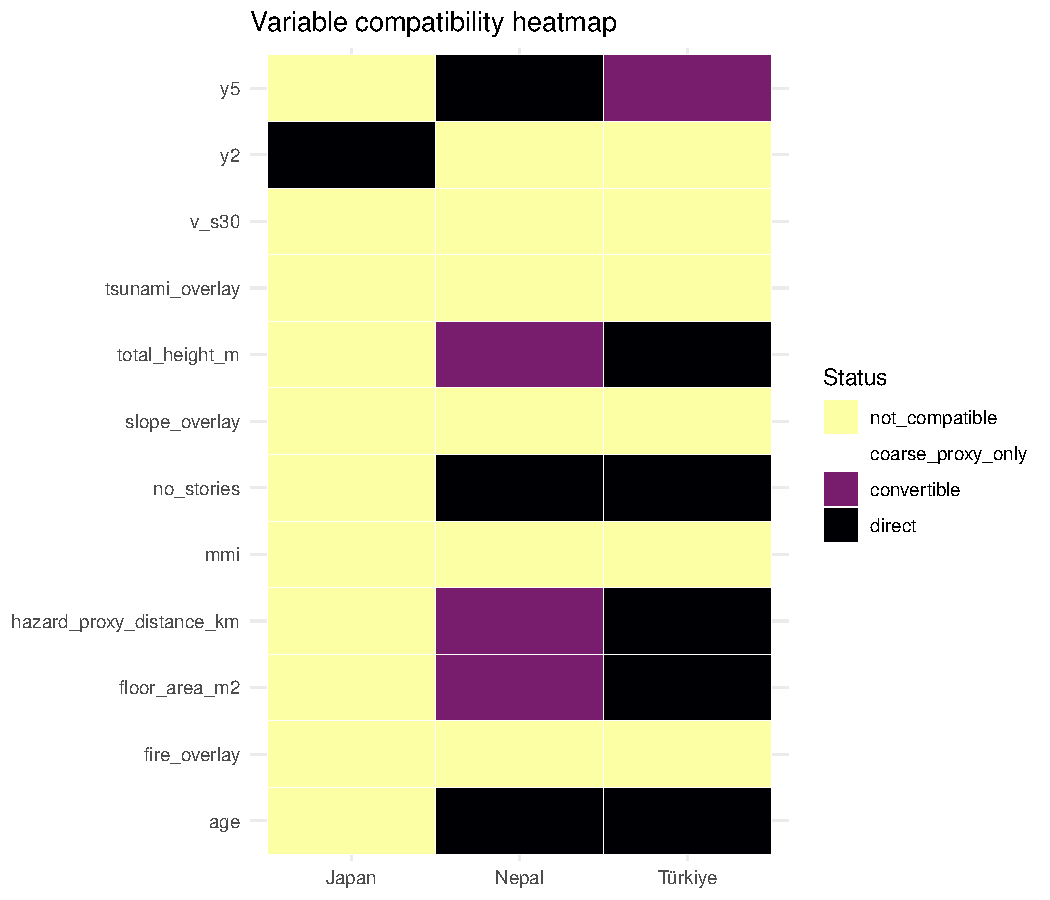
\includegraphics[width=0.85\linewidth]{figures/fig01_compatibility_heatmap.pdf}
\caption{Variable compatibility heatmap. Each row is a conceptual variable and each column is a country. Black indicates a directly available variable; purple indicates a variable available after a unit conversion or simple recoding; pale yellow indicates no usable analogue. The compatible block on the right (Nepal/T\"urkiye core: \texttt{age, no\_stories, floor\_area\_m2, total\_height\_m, hazard\_proxy\_distance\_km}) is the maximal intersection of the two survey-based inventories. Japan shares only the binary damage label \texttt{y2} as ``direct'' across the three datasets, illustrating its role as a measurement-regime contrast rather than a third symmetric training domain.}
\label{fig:compat-heatmap}
\end{figure}

\begin{figure}[!t]
\centering
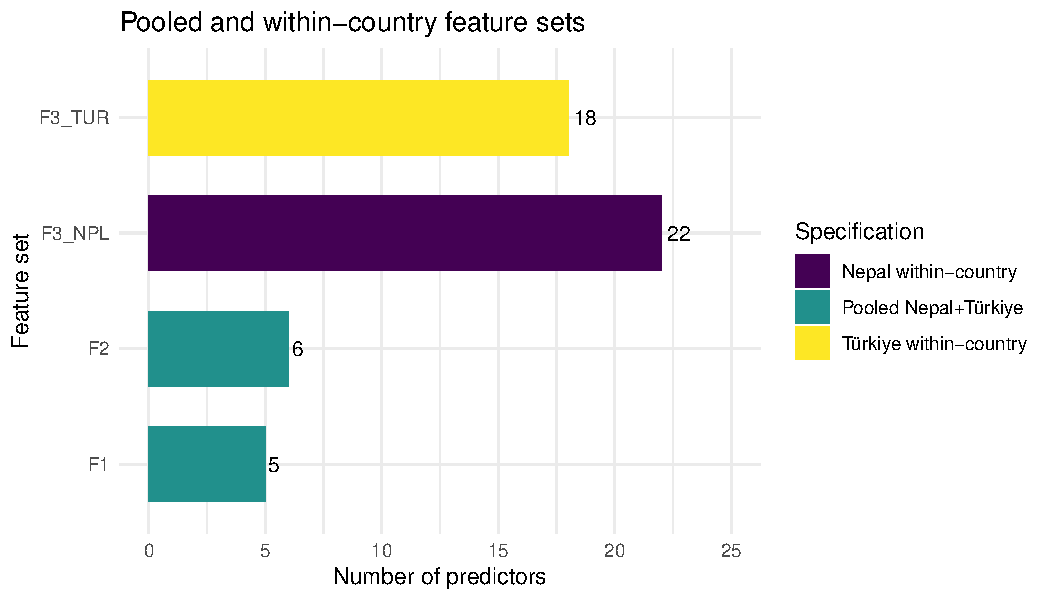
\includegraphics[width=0.85\linewidth]{figures/fig02_nested_feature_sets.pdf}
\caption{Nested harmonised feature sets used in the modelling and ablation experiments. $F_1$ and $F_2$ are pooled Nepal--T\"urkiye sets; $F_3$ denotes the country-specific full predictor sets used for within-country benchmarks.}
\label{fig:nested-sets}
\end{figure}

\subsection{What is the within-country upper bound?}
\label{subsec:results-within}

The within-country benchmarks establish the upper bound of what each modelling regime can deliver on the available data, before any harmonisation cost is paid. For Nepal, the 762{,}094-row inventory and the rich typological predictor set together permit Random Forest on $F_3^{\text{NPL}}$ to reach binary AUC $0.864$, accuracy $0.786$ and F1 $0.833$; on the five-class task the same model reaches accuracy $0.521$, balanced accuracy $0.472$ and macro-F1 $0.450$, clearly above the multinomial baseline and the proportional-odds ordinal baseline. The five-fold standard deviations are small in all metrics ($\le 0.002$), consistent with the very large sample. T\"urkiye, by contrast, inverts the model ordering at $n=242$: on $F_3^{\text{TUR}}$, logistic regression edges out Random Forest on binary AUC ($0.713$ vs.\ $0.700$), and the proportional-odds ordinal model achieves the highest five-class macro-F1 ($0.490$, against RF's $0.478$), because \texttt{polr} exploits the ordinal structure and 242 rows is too few for a tree ensemble to reliably outperform a structured baseline. The within-country Nepal and T\"urkiye results are reported in Tables~\ref{tab:turkiye-only} and~\ref{tab:nepal-only}; cells marked ``---'' are empty by construction. Japan supplies the remaining piece of the within-country picture under its own reference set $J_1$ (footprint area, USGS MMI, the three GSI overlays and the asset-level distance to the Noto epicentre): Random Forest reaches AUC $0.814$ (SD $0.004$), F1 $0.400$ and Brier $0.121$, while binary logistic regression on the same predictors collapses to AUC $0.643$ with severe-class sensitivity essentially zero (mean $0.0003$) and F1 $0.001$ --- a specification artefact of forcing an additive logit on an overlay-driven, non-linear hazard signal, not evidence about the discriminability of the data itself (Figure~\ref{fig:japan-within}, Table~\ref{tab:japan-within}). $J_1$ is reported only as a Japan-specific upper bound: it never enters the cross-country experiments in Section~\ref{subsec:results-transfer} because the GSI overlays have no Nepal or T\"urkiye analogue.


\begin{table}[!t]
\centering
\caption{T\"urkiye-only within-country benchmarks ($n=242$). Five-fold cross-validated mean. ``Logistic'' fits the binary task; ``Proportional odds'' fits the five-class ordinal task. Empty cells (``---'') reflect the model specification, not a missing computation. The neural-network five-class entry is flagged with $\dagger$ because, with only six grade-5 buildings in the dataset (Table~\ref{tab:samples}), macro-F1 is unstable across folds.}
\label{tab:turkiye-only}
\small
\begin{tabular}{l ccc ccc}
\toprule
& \multicolumn{3}{c}{\textbf{Five-class}}
& \multicolumn{3}{c}{\textbf{Binary}}\\
\cmidrule(lr){2-4}\cmidrule(lr){5-7}
Model & Acc & Bal.\ Acc & Macro-F1 & Acc & F1 & AUC \\
\midrule
Logistic / multinomial      & ---   & ---   & ---            & 0.682 & 0.772 & 0.713 \\
Proportional odds           & 0.661 & 0.608 & 0.490          & ---   & ---   & ---   \\
Random Forest               & 0.728 & 0.521 & 0.478          & 0.750 & 0.836 & 0.700 \\
Neural Network              & 0.721 & 0.721$^\dagger$ & 0.838$^\dagger$ & 0.713 & 0.825 & 0.608 \\
\bottomrule
\multicolumn{7}{l}{\footnotesize $^\dagger$ Macro-F1 unstable on rare-class folds; see text and Section~\ref{sec:discussion}.}
\end{tabular}
\end{table}

\begin{table}[!t]
\centering
\caption{Nepal-only within-country benchmarks ($n=762{,}094$). Five-fold cross-validated mean. Empty cells (``---'') reflect the model specification, not a missing computation. Five-fold standard deviations are $\le 0.002$ on every metric and are reported in the supplementary results file (\texttt{R/outputs/results/within\_country\_long.rds}).}
\label{tab:nepal-only}
\small
\begin{tabular}{l ccc ccc}
\toprule
& \multicolumn{3}{c}{\textbf{Five-class}}
& \multicolumn{3}{c}{\textbf{Binary}}\\
\cmidrule(lr){2-4}\cmidrule(lr){5-7}
Model & Acc & Bal.\ Acc & Macro-F1 & Acc & F1 & AUC \\
\midrule
Logistic / multinomial    & ---   & ---   & ---   & 0.737 & 0.809 & 0.768 \\
Proportional odds         & 0.432 & 0.344 & 0.300 & ---   & ---   & ---   \\
Random Forest             & \textbf{0.521} & \textbf{0.472} & \textbf{0.450} & \textbf{0.786} & \textbf{0.833} & \textbf{0.864} \\
Neural Network            & 0.423 & 0.357 & 0.355 & 0.740 & 0.810 & 0.744 \\
\bottomrule
\end{tabular}
\end{table}


\begin{figure}[!t]
\centering
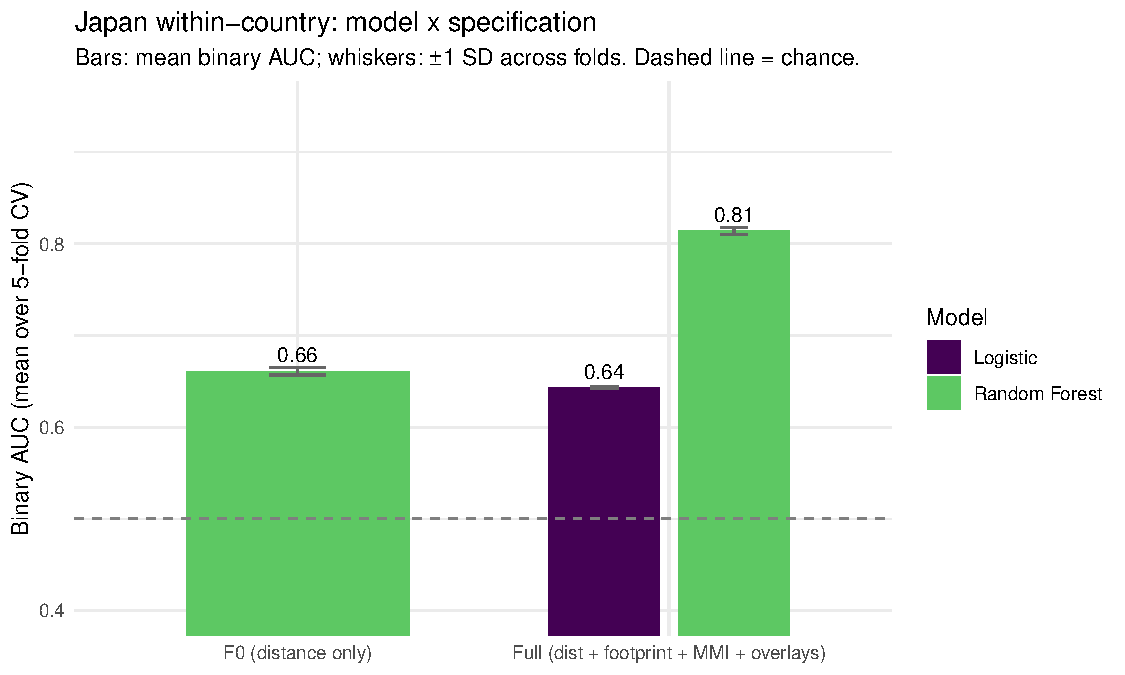
\includegraphics[width=0.85\linewidth]{figures/fig06_japan_within_country.pdf}
\caption{Japan within-country binary AUC by model and specification. ``Full'' is the within-country reference set $J_1$ (asset-level distance, footprint area, USGS MMI, GSI tsunami / fire / slope-failure overlays); ``$F_0$'' is the cross-country distance-only specification used in Section~\ref{subsec:results-transfer}. Bars are five-fold CV means; whiskers are $\pm 1$ SD across folds; the dashed line is the no-skill threshold. Logistic regression on $J_1$ collapses to predicting the majority class (severe-class sensitivity $\approx 0$, F1 $\approx 0.001$), so its AUC is informative about specification choice rather than data quality.}
\label{fig:japan-within}
\end{figure}

\begin{table}[!t]
\centering
\caption{Japan within-country binary AUC, five-fold cross-validated mean ($\pm$ SD) by model and specification. ``Full'' is $J_1$ (distance, footprint, MMI, GSI overlays); ``$F_0$'' is distance-only and is reported here only to anchor the harmonised-transfer comparison in Section~\ref{subsec:results-transfer}. Logistic regression is not run on $F_0$ because the univariate logit case is degenerate.}
\label{tab:japan-within}
\small
\begin{tabular}{l l l}
\toprule
\textbf{Model} & \textbf{Specification} & \textbf{Binary AUC} \\
\midrule
Random Forest      & Full ($J_1$)                    & $0.814 \pm 0.004$ \\
Logistic           & Full ($J_1$)                    & $0.643 \pm 0.001$ \\
Random Forest      & $F_0$ (distance only)           & $0.661 \pm 0.004$ \\
\bottomrule
\end{tabular}
\end{table}

\subsection{What happens under harmonised transfer?}
\label{subsec:results-transfer}

\paragraph{Nepal--T\"urkiye on $F_1$.} The Nepal--T\"urkiye transfer matrix in Table~\ref{tab:transfer-matrix} reports the central empirical finding of the paper on the harmonised core $F_1$. Pooling Nepal and T\"urkiye on $F_1$ and scoring on a held-out fold of the same pooled set reaches Random Forest binary AUC $0.827$, within $0.04$ of the best within-country Nepal fit. Adding the country indicator improves AUC by less than $0.001$, which means that within a random pooled holdout the country-level shift adds essentially no additional information beyond the harmonised predictor distributions. This pooled result should be read narrowly: a random pooled holdout is an interpolative evaluation in which both countries appear in train and test, so it demonstrates only that the harmonised feature table contains predictive signal under interpolation; it does not demonstrate deployability to an unseen country, and the small marginal value of the country indicator does not imply that country effects are absent. Direct cross-country transfer makes that point explicit: training on Nepal and scoring on T\"urkiye yields binary AUC $0.434$, while the reverse direction yields AUC $0.450$, both below the $0.5$ no-skill line. Below-chance AUC indicates that the model's learned risk ordering is systematically inverted in the target setting, consistent with predictor--damage relationships that change sign or shape across countries (Section~\ref{subsec:results-mechanism-and-simulation}); it is therefore stronger evidence of negative transfer than ``merely weak'' performance.

\begin{table}[!t]
\centering
\caption{Nepal--T\"urkiye train-to-test transfer matrix on $F_1$, Random Forest, binary AUC. Diagonal cells are pulled from the within-country results (\texttt{R/outputs/results/within\_country\_long.rds}); off-diagonal cells from the transfer experiment (\texttt{cross\_country\_transfer\_long.rds}). The held-out pooled cells correspond to a random fold within the Nepal+T\"urkiye pool (an interpolative evaluation, not a deployability test). The three-country counterpart on $F_0$ is reported in Table~\ref{tab:f0-transfer-matrix} and Figure~\ref{fig:transfer-heatmap}.}
\label{tab:transfer-matrix}
\small
\begin{tabular}{l ccc}
\toprule
& \multicolumn{3}{c}{\textbf{Test domain}} \\
\cmidrule(lr){2-4}
\textbf{Train domain} & Nepal & T\"urkiye & Pooled (held-out) \\
\midrule
Nepal              & \textbf{0.864} & \textbf{0.434} & ---   \\
T\"urkiye          & \textbf{0.450} & \textbf{0.700} & ---   \\
Pooled             & ---            & ---            & 0.827 \\
Pooled w/o country & ---            & ---            & 0.828 \\
\bottomrule
\end{tabular}
\end{table}

\paragraph{Three-country $F_0$: within-country baselines and pooled fit.} The reduced-specification stress test asks whether the same conclusion holds when Japan is added to the modelling step under the maximally reductive distance-only specification $F_0$ (Section~\ref{subsec:methods-compatibility}). The within-country $F_0$ baselines reproduce a familiar pattern: Random Forest reaches AUC $0.770$ on Nepal ($n=762{,}094$), $0.583$ on T\"urkiye ($n=242$, SD $0.050$, with the relatively high SD reflecting the small T\"urkiye fold size) and $0.661$ on Japan. When the three countries are pooled on $F_0$, the three-country Random Forest reaches AUC $0.789$ with a country indicator and $0.785$ without, with five-fold standard deviations $\le 0.001$ in each case. The pooled fit therefore beats the strongest within-country $F_0$ baseline by approximately $0.02$, and the marginal value of the explicit country indicator over the implicit country distribution captured by the predictor itself is $\le 0.005$. As above, the pooled result should be read as an interpolative evaluation; it does not show that a pooled three-country $F_0$ model would deploy to an unseen country. Figure~\ref{fig:f0-pooled-vs-within} reports both panels side by side; Table~\ref{tab:f0-pooled} gives the numbers.

\begin{figure}[!t]
\centering
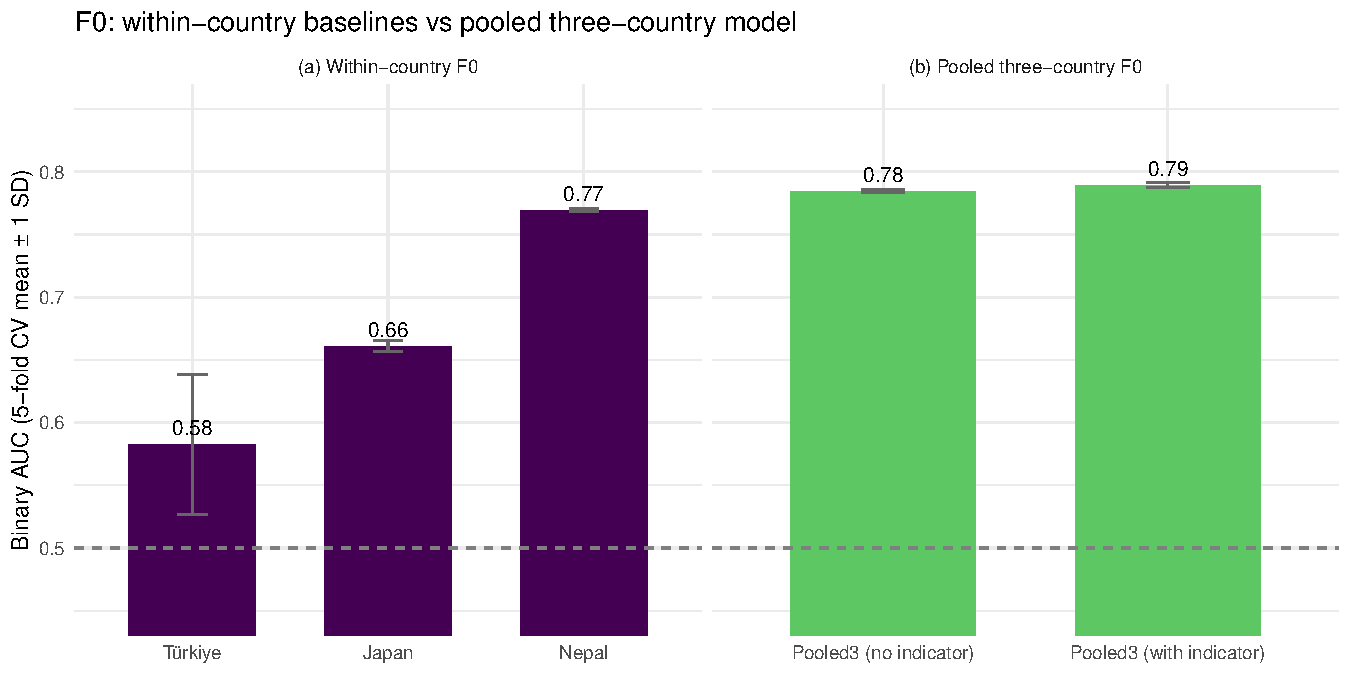
\includegraphics[width=0.95\linewidth]{figures/fig08_pooled_vs_within_F0.pdf}
\caption{Three-country distance-only ($F_0$) Random Forest, binary AUC. (a) Within-country baselines for Nepal, T\"urkiye and Japan. (b) Pooled three-country fits with and without a categorical country indicator. Bars are five-fold cross-validated means with $\pm 1$ SD whiskers; the dashed line is the no-skill threshold. The pooled three-country fit improves over the strongest within-country baseline (Nepal at $0.77$) by approximately $0.02$, and adding the country indicator is essentially neutral.}
\label{fig:f0-pooled-vs-within}
\end{figure}

\begin{table}[!t]
\centering
\caption{Within-country and pooled three-country $F_0$ Random Forest results. Five-fold cross-validated binary AUC, mean $\pm$ SD. The pooled fits use \texttt{rsample::vfold\_cv} stratified by \texttt{country}, so each fold contains all three countries.}
\label{tab:f0-pooled}
\small
\begin{tabular}{l l l}
\toprule
\textbf{Country / pool} & \textbf{Specification} & \textbf{Binary AUC} \\
\midrule
Nepal                                 & $F_0$, RF                        & $0.770 \pm 0.001$ \\
T\"urkiye                             & $F_0$, RF                        & $0.583 \pm 0.050$ \\
Japan                                 & $F_0$, RF                        & $0.661 \pm 0.004$ \\
\midrule
Pooled three-country (with indicator) & $F_0$, RF, $+$ \texttt{country}  & $0.789 \pm 0.001$ \\
Pooled three-country (no indicator)   & $F_0$, RF                        & $0.785 \pm 0.001$ \\
\bottomrule
\end{tabular}
\end{table}

\paragraph{$3\times 3$ transfer on $F_0$.} The three-country transfer matrix in Figure~\ref{fig:transfer-heatmap} and Table~\ref{tab:f0-transfer-matrix} converts the pooled $F_0$ result into a deployability-style test: each off-diagonal cell is a single train-on-A / test-on-B fit. Off-diagonal performance is uniformly weak. Only T\"urkiye-trained $\rightarrow$ Nepal-tested clearly clears the no-skill line (AUC $0.635$); the remaining five off-diagonal cells range from marginal (Nepal$\rightarrow$T\"urkiye $0.538$, Japan$\rightarrow$Nepal $0.495$, Japan$\rightarrow$T\"urkiye $0.478$) to clearly negative (Nepal$\rightarrow$Japan $0.428$, T\"urkiye$\rightarrow$Japan $0.365$). The Japan column is particularly hard: distance signals trained in Nepal or T\"urkiye actively misclassify Japan because the Noto event has a very different distance--damage shape from the Gorkha and Pazarc{\i}k--Elbistan events (Section~\ref{subsec:results-mechanism-and-simulation}). This is consistent with the Nepal--T\"urkiye $F_1$ transfer failure documented above, but on a strictly weaker specification, which rules out the alternative reading that the $F_1$ failure was driven by harmonisation noise on the structural attributes specifically: even when only one jointly observable predictor is used, transfer fails. The T\"urkiye diagonal cell sits well above its five-fold CV mean ($0.776$ in the single 80/20 split, $0.583$ on average across folds): at $n=242$ the T\"urkiye estimate is intrinsically unstable, so the diagonal cells in this matrix should be read as comparison anchors for the off-diagonal transfer cells rather than as best estimates of within-country performance, which are reported in Table~\ref{tab:f0-pooled}.

\begin{figure}[!t]
\centering
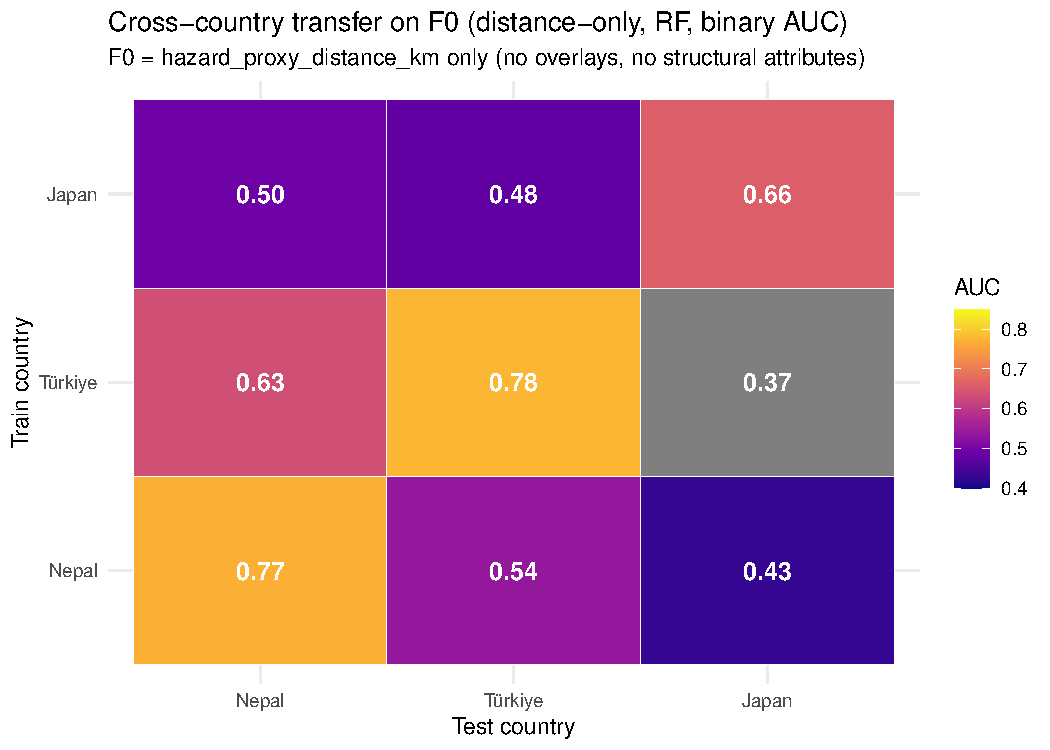
\includegraphics[width=0.85\linewidth]{figures/fig03_transfer_heatmap.pdf}
\caption{Three-country cross-country transfer on $F_0$ (distance-only), Random Forest, binary task, AUC. Each cell is a single train-on-A / test-on-B fit; diagonal cells are the corresponding within-country 80/20 splits and act as comparison anchors for the off-diagonal transfer cells. The Türkiye diagonal ($0.78$) sits well above its five-fold CV mean of $0.583$ (Table~\ref{tab:f0-pooled}) because at $n=242$ the within-country estimate is unstable across splits. Off-diagonal transfer is uniformly weak: only T\"urkiye$\rightarrow$Nepal ($0.64$) clearly clears the $0.5$ no-skill line; Nepal$\rightarrow$T\"urkiye ($0.54$), Japan$\rightarrow$Nepal ($0.50$), Japan$\rightarrow$T\"urkiye ($0.48$), Nepal$\rightarrow$Japan ($0.43$) and T\"urkiye$\rightarrow$Japan ($0.37$) range from marginal to negative.}
\label{fig:transfer-heatmap}
\end{figure}

\begin{table}[!t]
\centering
\caption{Three-country $F_0$ train-to-test transfer matrix, Random Forest, binary AUC. Diagonal cells come from the single 80/20 train-test split used inside the transfer experiment, not from five-fold CV; they should be read as comparison anchors for the off-diagonal cells, not as best within-country estimates. The corresponding five-fold CV within-country baselines are reported in Table~\ref{tab:f0-pooled}. Bold cells are below the $0.5$ no-skill line.}
\label{tab:f0-transfer-matrix}
\small
\begin{tabular}{l ccc}
\toprule
& \multicolumn{3}{c}{\textbf{Test country}} \\
\cmidrule(lr){2-4}
\textbf{Train country} & Nepal & T\"urkiye & Japan \\
\midrule
Nepal     & 0.770          & 0.538          & \textbf{0.428} \\
T\"urkiye & 0.635          & 0.776          & \textbf{0.365} \\
Japan     & \textbf{0.495} & \textbf{0.478} & 0.659 \\
\bottomrule
\end{tabular}
\end{table}

\paragraph{Overlap-ablation curve.} The overlap-ablation experiment in Figure~\ref{fig:ablation} traces the same harmonisation logic on the Nepal--T\"urkiye pool: as the harmonised core is reduced from $K_5$ to $K_1$, Random Forest binary AUC declines from $0.828$ to $0.770$, logistic regression from $0.686$ to $0.622$ and the neural network from $0.769$ to $0.659$. The within-model decline is real but modest in the empirical setting because the dominant single predictor, the hazard-distance proxy, already carries most of the within-pool signal. The five-class macro-F1 panel contains a metric artefact at $K_1$, where the proportional-odds model collapses to predicting the modal class and the macro average runs over only the few classes that appear in the test fold; the inflated value is interpreted as a metric pathology rather than as a substantive result.

\begin{figure}[!t]
\centering
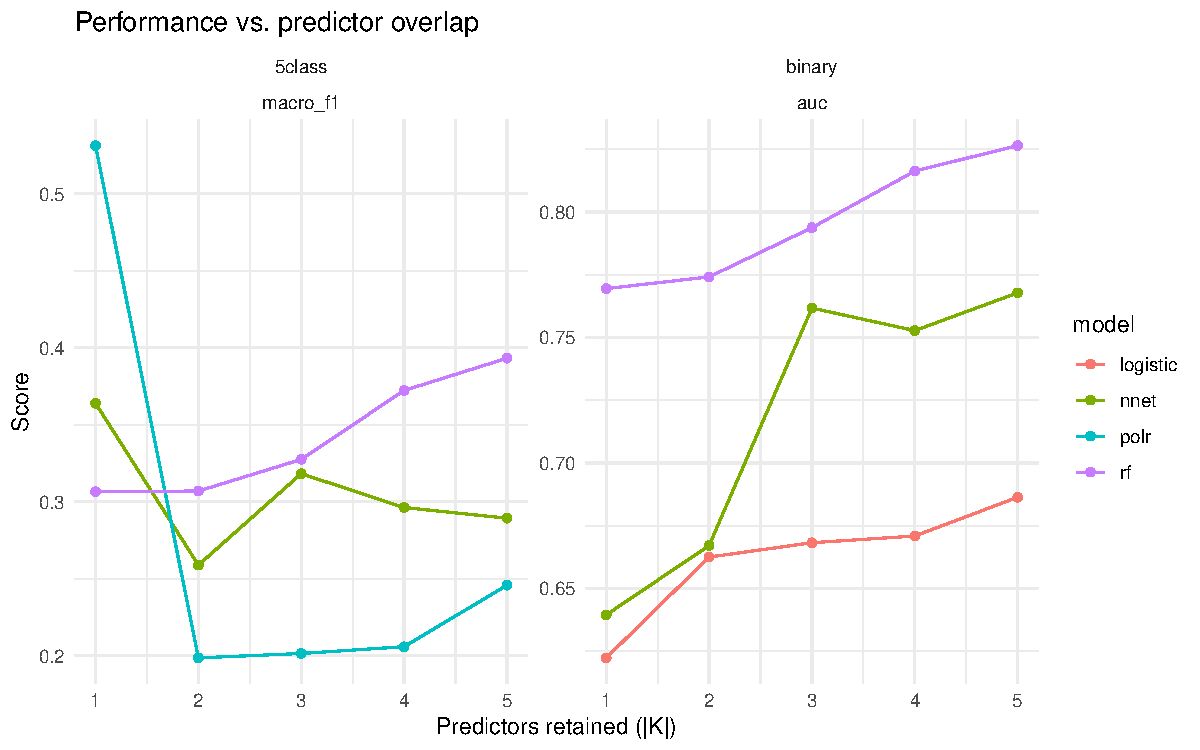
\includegraphics[width=0.95\linewidth]{figures/fig04_overlap_ablation.pdf}
\caption{Overlap-ablation curves on the Nepal--T\"urkiye pool. The horizontal axis is the number of harmonised predictors retained ($K_1$ to $K_5$); each line is a model family. For binary AUC, all model families decline gently as overlap shrinks. The five-class macro-F1 panel contains a metric artefact at $K_1$ for proportional odds (see text); that data point should not be over-interpreted.}
\label{fig:ablation}
\end{figure}

\subsection{Why does transfer fail?}
\label{subsec:results-mechanism}

\paragraph{Class-wise diagnostics for the within-country fits.} The diagnostic confusion matrices show that the headline discrimination metrics hide important class-wise behaviour. For the Nepal binary Random Forest, the held-out confusion matrix gives accuracy $0.757$, severe-class sensitivity $0.839$, specificity $0.630$ and severe-class F1 $0.807$. For T\"urkiye, the corresponding binary matrix gives accuracy $0.735$, severe-class sensitivity $0.788$, specificity $0.625$ and severe-class F1 $0.800$. The five-class matrices are less stable: Nepal reaches accuracy $0.477$ and Cohen's $\kappa=0.287$, but class-wise sensitivity remains weak for DG2 and DG3, while DG5 is much better identified; T\"urkiye reaches apparent five-class accuracy $0.673$, but this is below the no-information rate of $0.735$ and the sensitivities for DG2, DG3 and DG5 are zero in the held-out fold. A grouped Nepal cross-validation by \texttt{vdcmun\_id} further reduces the binary Random Forest estimate from the random-split AUC of $0.864$ to mean AUC $0.785$ (SD $0.054$), with accuracy $0.732$ (SD $0.048$), F1 $0.785$ (SD $0.042$) and Brier score $0.181$ (SD $0.026$): the within-country signal remains substantial under grouped geographic splitting, but the random split is likely optimistic and should not be read as a strict out-of-region generalisation estimate.

\paragraph{Sign and shape changes in the harmonised predictors.} The transfer failure under both $F_1$ and $F_0$ is substantive rather than merely statistical: harmonised predictors plausibly encode different physical relationships in different countries. Number of storeys is largely a wealth and construction-quality proxy in Nepal but a height and ductility-demand proxy in T\"urkiye; age proxies for material and mortar quality in Nepal but for seismic-code era in T\"urkiye; and the distance proxy operates with different decay constants because the events differ in magnitude, source mechanism, attenuation, soil conditions and directivity. Country-specific variable-importance rankings, simple logistic marginal effects and country-stratified partial-dependence curves (supplementary diagnostics in \texttt{R/code/09\_diagnostics.R}) support this reading. The sign diagnostics show that common feature names do not always correspond to common operational meaning: age is positive and precise in Nepal but small, negative and non-significant in T\"urkiye; floor area is negative in Nepal but positive, though imprecisely estimated, in T\"urkiye; and increasing \texttt{no\_stories} lowers predicted severe-damage probability in Nepal while raising it in T\"urkiye.

\paragraph{Distance--damage curves explain the negative Japan cells.} The mechanism behind the off-diagonal Japan cells of the $F_0$ transfer matrix is visible in the country-specific marginal severity-by-distance curves on $F_0$ (Figure~\ref{fig:distance-damage-curve}). Nepal shows a comparatively flat, monotonic decay of the empirical severe-damage rate with distance, consistent with a regional inventory whose hazard variable is itself a coarse district-level distance aggregate. T\"urkiye starts at a much higher severe-damage rate at near-source distances and drops steeply but with substantial bin-to-bin volatility, consistent with $n=242$. Japan exhibits a shape that is qualitatively different from both: a low overall severe-damage rate (binary base rate $0.199$, vs.\ $0.603$ for Nepal and $0.649$ for T\"urkiye) with a pronounced decay only at intermediate distances, dominated by tsunami- and ground-failure-driven near-source damage that is not captured by epicentral distance alone. A model trained on Nepal therefore expects severe damage at most short distances and over-predicts on the lower-base-rate Japanese inventory; a model trained on T\"urkiye expects steep distance decay and over-predicts at long distances on Japan. The negative cells in the transfer matrix are thus not a numerical artefact but a direct consequence of these incompatible distance--damage shapes.

\begin{figure}[!t]
\centering
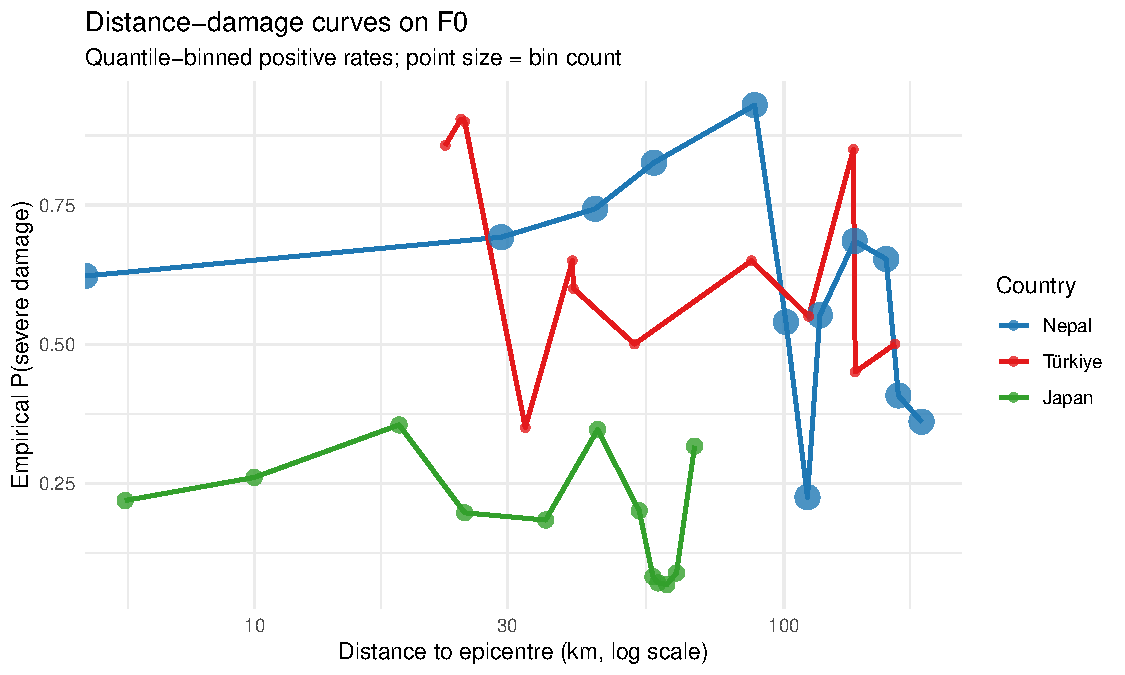
\includegraphics[width=0.85\linewidth]{figures/fig07_distance_damage_curve.pdf}
\caption{Country-specific marginal distance--damage curves on $F_0$. Each line is the empirical severe-damage rate within country-specific quantile bins of asset-level distance to source; point size scales with bin count. Distance is plotted on a log scale because the three countries cover very different distance ranges ($\sim$1--80~km for Japan, district-aggregated up to $\sim$300~km for Nepal). Diverging shapes between Japan and the two survey-based inventories explain why the off-diagonal Japan cells of the $F_0$ transfer matrix sit below the $0.5$ no-skill line.}
\label{fig:distance-damage-curve}
\end{figure}

\paragraph{Calibration of the pooled binary Random Forest.} The pooled Nepal--T\"urkiye binary Random Forest is moderately but not perfectly calibrated. The Brier score is $0.165$, and the calibration curve (supplementary diagnostic produced by \texttt{R/code/09\_diagnostics.R}) follows the diagonal in the central probability range while showing visible deviations at the extremes, where fewer observations are available. This matters for DRR applications because a model used for inspection prioritisation or reconstruction triage would normally be deployed as a probability-producing decision aid rather than only as a ranker. The AUC results should therefore be interpreted alongside the calibration diagnostic: the pooled model discriminates reasonably well within the pooled Nepal--T\"urkiye holdout, but probability estimates should be recalibrated before operational deployment.

% NOTE: The country-stratified partial-dependence figure
% (fig06_partial_dependence_by_country.pdf) and pooled-RF calibration
% figure (fig07_calibration_pooled_rf.pdf) are produced by
% R/code/09_diagnostics.R but are not currently included in the paper:
% the corresponding files are not in paper/figures/, and fig06/fig07
% are now used by the Japan within-country and distance--damage figures.
% To re-introduce them, regenerate under free figure numbers and add
% \begin{figure}...\end{figure} blocks here.

\subsection{Does the simulation support the interpretation?}
\label{subsec:results-mechanism-and-simulation}

The simulation answers RQ3 within its scenario grid (Section~\ref{subsec:methods-simulation}) by holding the data-generating process fixed while varying compatibility regime and model class. Figure~\ref{fig:sim-surface} shows binary AUC as a function of \texttt{p\_shared} and \texttt{sigma\_measure}: at full overlap with no measurement error, binary AUC reaches approximately $0.95$; at \texttt{p\_shared} $=0.2$, the model degrades to near-random scores irrespective of measurement noise. The two-way variance decomposition reported in Figure~\ref{fig:sim-variance} is the more compact summary. For binary AUC, the compatibility regime explains $51.8\%$ of the variance against $1.9\%$ for model family, a regime-to-model variance ratio of approximately $27{:}1$. For five-class macro-F1, the corresponding shares are $56.2\%$ and $0.3\%$, approximately $187{:}1$. For accuracy the order inverts, with model family explaining $24.7\%$ against $5.4\%$ for regime, because accuracy rewards over-prediction of the majority class and therefore confounds discrimination quality with class balance. Taken together, for discrimination-oriented metrics the compatibility regime dominates the choice of model class by an order of magnitude or more in the simulated grid, while for accuracy alone the picture is more nuanced. The simulation is sensitive to the chosen scenario grid and to the shared/country-specific coefficient distribution; the variance shares should therefore be read as bounds under plausible conditions rather than as universal estimates.

\begin{figure}[!t]
\centering
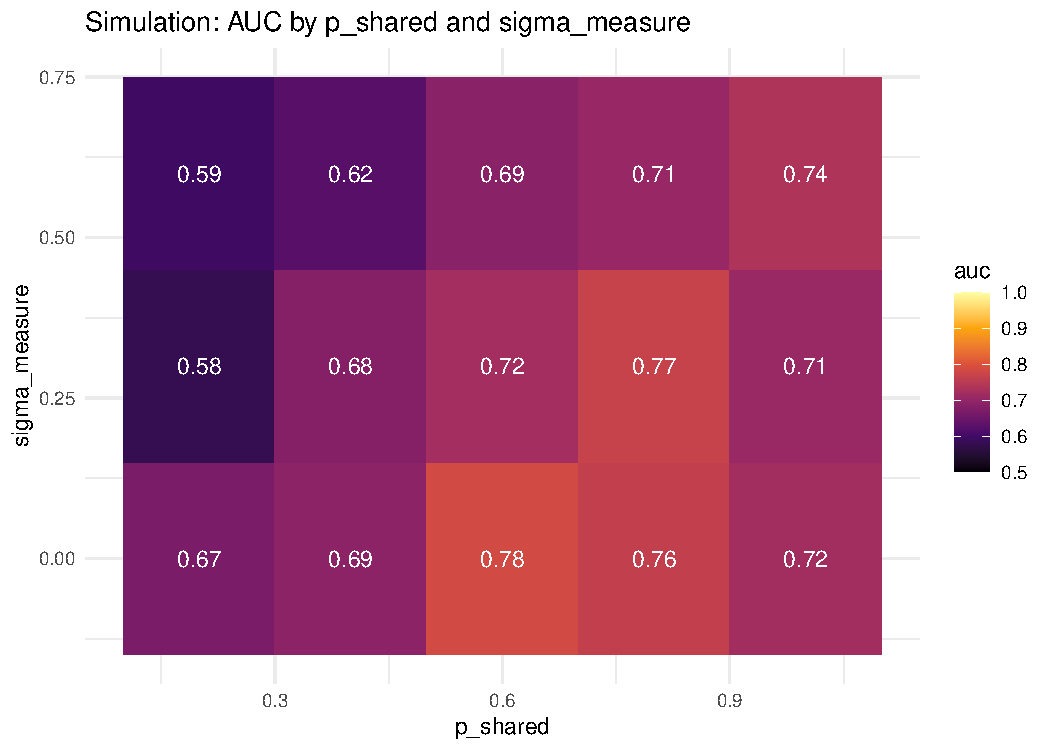
\includegraphics[width=0.85\linewidth]{figures/fig05a_sim_surface.pdf}
\caption{Simulation results, binary AUC averaged over models, repetitions and label-noise scenarios. AUC degrades systematically as the share of shared predictors (\texttt{p\_shared}) shrinks and as country-specific measurement error (\texttt{sigma\_measure}) grows.}
\label{fig:sim-surface}
\end{figure}

\begin{figure}[!t]
\centering
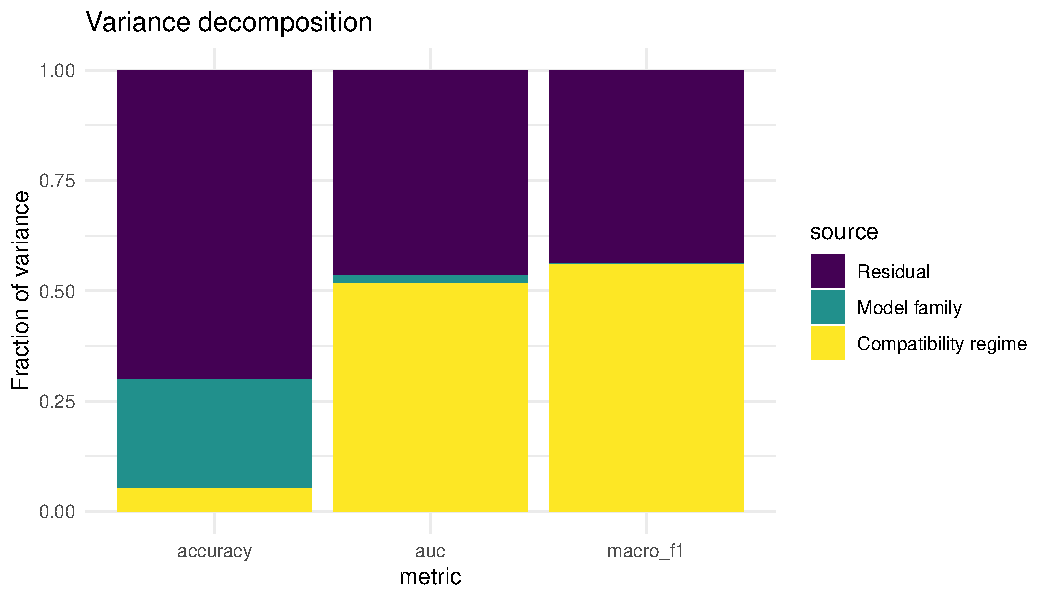
\includegraphics[width=0.7\linewidth]{figures/fig05b_variance_decomp.pdf}
\caption{Variance decomposition from the simulation. For AUC and macro-F1 the compatibility regime explains roughly $0.52$ and $0.56$ of the variance respectively, against $0.02$ and $0.003$ for model family; for accuracy the picture inverts.}
\label{fig:sim-variance}
\end{figure}

% =====================================================================
\section{Discussion}
\label{sec:discussion}
% =====================================================================

\paragraph{Central finding.} The results support one main point: under the harmonisation regime examined here, cross-country earthquake damage modelling is constrained more by data compatibility than by the choice among standard classifiers. This is a claim about \emph{this} harmonised core on \emph{these} three earthquakes, not a universal claim about machine learning. Within-country, the same algorithms recover meaningful predictive signal --- Nepal reaches Random Forest binary AUC $0.864$, T\"urkiye logistic regression $0.713$, Japan within-country RF on $J_1$ $0.814$ --- and pooled fits on the harmonised cores remain serviceable as interpolative evaluations (Nepal+T\"urkiye on $F_1$, AUC $0.827$; three-country $F_0$, $0.789$). The point is not that the algorithms have failed; it is that direct $A \rightarrow B$ deployment fails for almost every country pair examined, with five of the six off-diagonal $F_0$ cells at or below chance and the two $F_1$ off-diagonals (Nepal$\rightarrow$T\"urkiye, T\"urkiye$\rightarrow$Nepal) clearly negative. Adding a country indicator changes pooled AUC by less than $0.001$, but this does not show that country effects are absent: it only shows that within a random pooled split source differences are already absorbed by the observed predictor distributions, an interpolative evaluation rather than a deployability test.

\paragraph{Mechanism.} The substantive interpretation is that the shared feature space is too thin to carry the same physical meaning across countries. Harmonised predictor names mask different operational referents: number of storeys is a wealth and construction-quality proxy in Nepal but a height and ductility-demand proxy in the T\"urkiye reinforced-concrete sample; age proxies for material quality in one context and seismic-code era in the other; and distance-to-source is only a weak hazard substitute when earthquakes differ in magnitude, rupture geometry, attenuation, soil conditions and directivity. The country-stratified distance--damage curves on $F_0$ make this visible: each country has its own distance--severity shape, so a single jointly observable predictor cannot substitute for a harmonised inventory. Below-chance off-diagonal AUCs are therefore best understood as evidence that the learned risk ordering is systematically inverted in the target setting, not as merely noisy estimates.

\paragraph{Relation to existing literature.} These results sit between two recent reference points. \citet{patten2024datadriven} reach AUC near $0.93$ on a 2023 T\"urkiye holdout by training a multi-impact damage model on roughly $370{,}000$ buildings across 26 earthquakes in 61 countries; their setting is what cross-country damage modelling can look like \emph{after} a substantial harmonisation programme has been carried out. \citet{ghimire2024host} report that out-of-region accuracy across a different multi-country corpus is bounded by data quality and contextual similarity rather than classifier sophistication; their result is that transfer fails across heterogeneous datasets. The present paper sits between the two and supplies a mechanism: in the absence of large-scale harmonisation, the common feature space is too thin and the harmonised predictors carry country-specific operational meanings, so transfer fails not because algorithms are weak but because the data infrastructure is. With respect to the standardisation literature, GEM's exposure taxonomies and GED4ALL building classification \citep{silva2022buildingclass, yepes2023exposure} provide the pre-event side of harmonised data infrastructure; the present paper argues that the missing layer is the corresponding post-event damage-survey layer, and that minimum-variable proposals such as Table~\ref{tab:min-core} are the operational form that layer should take. The simulation gives this argument a controlled setting: \emph{within} the scenario grid, for discrimination-oriented metrics the compatibility regime explains substantially more variance than the choice among standard classifiers (Section~\ref{subsec:results-mechanism-and-simulation}). The variance shares are not universal coefficients --- they are specific to the simulated grid --- but they bound the relative contribution of regime and model under plausible conditions, which is what RQ3 requires.

\paragraph{Operational policy pathways.} The minimum variable core proposed in Table~\ref{tab:min-core} is deliberately small, so it is not a wish list and can plausibly be embedded in operational instruments. Concretely, this means: national post-event survey forms (e.g.\ AeDES-style instruments) updated to require the eight families in Table~\ref{tab:min-core} as mandatory fields rather than optional ones; engineering reconnaissance protocols (ACI~133, EERI/GEER post-earthquake reports) extended to record the same fields under the same units and provenance metadata; humanitarian damage-assessment templates (REACH, IFRC, OCHA) aligned to the same minimum core so that humanitarian and engineering surveys produce interoperable rather than parallel records; mandatory provenance for hazard-intensity derivation (which ShakeMap version, which strong-motion network) attached to every record; versioned mappings from national typologies to GED4ALL and from national damage scales to EMS-98, treated as living artefacts rather than one-off harmonisation exercises; open exposure and vulnerability databases (GED4ALL, GEM-EXP) updated to consume Table~\ref{tab:min-core}-compliant records; and a Sendai Monitor reporting profile that exposes the minimum core to UNDRR Targets A--D, so that national post-event surveys are reusable for cross-country loss accounting rather than only for domestic recovery management. The audience for this layer is therefore not only researchers and modellers; it includes national disaster management agencies, post-earthquake reconnaissance teams, reconstruction authorities, humanitarian damage-assessment actors and catastrophe-modelling groups.

\paragraph{Limitations.} Several limitations bound the interpretation, grouped by source.
\textit{Data limitations:} the Nepal and T\"urkiye datasets are highly asymmetric in size ($\sim$762k vs.\ 242 records); the T\"urkiye sample is restricted to reinforced-concrete buildings and is not nationally representative; the Nepal hazard variable is a coarse district-level distance proxy rather than a harmonised shaking-intensity measure; and Japan changes the measurement regime altogether (remote-sensing footprint geometry plus GSI overlays), which is precisely why $J_1$ is reported only as a within-country reference and Japan enters cross-country experiments only through $F_0$.
\textit{Target limitations:} the binary severe-versus-non-severe target collapses the ordinal grade ladder and may smooth over operationally important grade distinctions; ordinal damage labels differ in timing, original purpose (engineering reconnaissance vs.\ remote sensing vs.\ recovery management) and collection protocol, so they are not all observations of the same latent severity process.
\textit{Model limitations:} only standard classifiers (logistic / multinomial, proportional odds, Random Forest, feed-forward NN) are evaluated, with limited hyper-parameter tuning, and the cross-country transfer protocol uses a single train-to-test direction per country pair; deep, image-based or domain-adaptive transfer methods may produce a different picture.
\textit{External-validity limitations:} the empirical conclusions are based on three earthquakes (Gorkha 2015, the 2023 T\"urkiye sequence, Noto 2024) and four-to-five datasets; the negative-transfer pattern is consistent with the broader multi-country evidence \citep{ghimire2024host} but should not be read as a universal estimate.
\textit{Simulation limitations:} the latent severity model is stylised, the scenario grid is pre-specified rather than calibrated to any one country, and the variance shares are sensitive to that grid and to the shared/country-specific coefficient distribution.
These limitations define the scope of the claim rather than overturning it: on the harmonised core available here, data infrastructure is the main bottleneck, and the minimum core in Table~\ref{tab:min-core} is the proposed operational response.


\begin{table}[!t]
\centering
\caption{Proposed minimum standardised asset-level variable core for post-event surveys. Intended users include national disaster management agencies, post-earthquake reconnaissance teams, engineering survey teams, reconstruction authorities, humanitarian damage-assessment actors, catastrophe-modelling groups and the
international organisations supporting exposure and vulnerability data standards. The variables are deliberately earthquake oriented but most are hazard-agnostic; with the addition of hazard-specific intensity proxies (e.g.\ flood depth, wind speed, ash load), the same core would extend to a multi-hazard exposure schema, in line with the GED4ALL building classification system \citep{silva2022buildingclass}}
\label{tab:min-core}
\small
\begin{tabularx}{\linewidth}{l X X X}
\toprule
\textbf{Variable group} & \textbf{Minimum variable} & \textbf{Why it matters} & \textbf{Collection recommendation} \\
\midrule
Identifier         & Persistent asset ID                                   & Linkage across surveys, registries and exposure databases & Issue at first survey, retain across events \\
Geolocation        & Point lat/lon (and footprint polygon when available)  & Spatial join with hazard, exposure and DRR overlays      & Survey GPS or geocoded address \\
Hazard intensity   & PGA, PGV, SA($T_1{=}1\,$s), MMI at asset location     & Comparable cross-event exposure                          & Derive from ShakeMap/USGS/national strong-motion network and record provenance \\
Geometry           & Year built, no.\ storeys, total height (m), floor area (m$^2$) & Core size and age determinants                  & Standardised form fields, SI units only \\
Structural system  & GED4ALL category \citep{silva2022buildingclass}       & Cross-country typology comparability                      & Map national typology to GED4ALL on collection \\
Site condition     & $V_{s30}$ (m/s) or NEHRP/Eurocode site class          & Local site amplification                                  & National $V_{s30}$ map look-up; record method \\
Damage label       & EMS-98 ordinal grade (DG1--DG5) plus binary severity flag & Comparable training target                            & Train field assessors on EMS-98; release both labels \\
Protocol metadata  & Survey type, inspection date, verification status      & Reproducibility, weighting, audit trail                  & Mandatory metadata fields in survey instrument \\
\bottomrule
\end{tabularx}
\end{table}

% =====================================================================
\section{Conclusion}
\label{sec:conclusion}
% =====================================================================

This study examined whether existing post-disaster earthquake damage datasets can support transferable asset-level modelling. The richer empirical experiment used Nepal and T\"urkiye, because both provide survey-based inventories with ordinal damage labels; Japan was then re-introduced as a reduced-specification stress test on the distance-only specification $F_0$, with country-specific hazard overlays deliberately excluded from any shared model.
The results support a single conclusion. Within-country and pooled Nepal--T\"urkiye models recover meaningful predictive signal, but direct cross-country transfer falls below the 0.5 AUC benchmark in both directions on the harmonised core examined here. The Japan stress test extends this picture: within country, Japan has a defensible binary signal under its full specification ($J_1$ Random Forest AUC $0.81$), but most of that signal does not survive the move to the cross-country distance-only specification ($F_0$ AUC $0.66$); the pooled three-country $F_0$ fit reaches AUC $0.79$ with essentially no marginal value from the country indicator; and the $3\times 3$ $F_0$ transfer matrix is dominated by below-chance off-diagonal cells. The controlled simulation reinforces this reading: for discrimination metrics, the compatibility regime explains roughly an order of magnitude more variance than the choice among standard classifiers. Read alongside \citet{patten2024datadriven}, who reach high AUC on a much larger harmonised global corpus, and \citet{ghimire2024host}, who report similar transfer failure across heterogeneous datasets, the present findings indicate that cross-country damage modelling is feasible, but only when the underlying data infrastructure carries comparable measurement across contexts.
These findings carry a direct DRR-policy implication. Sendai Framework Priority 1 and Sendai Monitor Targets A--D both presume loss data that are consistent across countries; the minimum standardised asset-level core proposed in Table~\ref{tab:min-core} is one concrete route to that consistency. To convert the recommendation into practice, the core should be aligned with the GEM/GED4ALL exposure schema \citep{silva2022buildingclass, yepes2023exposure} and with national reconnaissance protocols (e.g.\ ACI~133, EERI, GEER, Kathmandu Living Labs, AFAD), and adopted as a metadata standard for post-event surveys submitted to the UNDRR Sendai Monitor. Although the present study is earthquake-specific, the structure of the proposed core is hazard-agnostic and could be extended toward multi-hazard exposure-and-impact harmonisation.
The remaining caveats mean that the numerical results should be read as evidence about transfer under the available harmonised core, not as universal performance estimates for Nepal, T\"urkiye or Japan. The consequence is practical: the next step is to embed Table~\ref{tab:min-core} in reconnaissance protocols, exposure standards and Sendai Monitor reporting, so that future models are trained on reusable cross-country data infrastructure rather than on retrospective harmonisation alone.

% =====================================================================
\section*{Declarations}
\addcontentsline{toc}{section}{Declarations}
% =====================================================================

\paragraph{Generative AI.}

During the preparation of this work, generative AI was used to support language editing, structural revision, and the drafting of reviewer-response material. The tool was not used to generate original empirical results, conduct unsupervised data analysis, or make final scientific interpretations. After using this tool, the author reviewed, verified, and edited the content as needed and takes full responsibility for the content of the published article.

\paragraph{Funding.} No specific funding was received for this
work.

\paragraph{Competing interests.} The author declares no competing
interests.


\paragraph{Data availability.} The Nepal post-Gorkha building
inventory is publicly available through the source release of
\citet{ghimire2022nepal}. The T\"urkiye ACI~133 reconnaissance
dataset is described in \citet{hariri2025turkiye} and is available
under the access conditions of that source. The Japan 2024 Noto
Peninsula building damage dataset is publicly available from the
Earth System Science Data release of \citet{vescovo2025noto}.

\paragraph{Code availability.} All harmonisation, modelling,
ablation and simulation code is implemented in R as a series of
nine numbered scripts; the code base
accompanying this paper is available from the author on request.

\paragraph{Acknowledgements.} The author thanks the producers and
maintainers of the three source datasets for making the
underlying data available.

% =====================================================================
\bibliographystyle{plainnat}
\bibliography{references}
\newpage
\appendix
% =====================================================================
\section*{Appendix A: Variable importance tables retained for
backward comparability}
\addcontentsline{toc}{section}{Appendix A: Variable importance tables}

\begin{table}[!h]
\centering
\caption{T\"urkiye-only, five-class task: top variable-importance
metrics (Random Forest).}
\label{tab:imp-turkiye-5}
\small
\begin{tabular}{l r}
\toprule
Variable & Importance drop \\
\midrule
\texttt{m7\_5\_sa\_t1}                      & 0.009398 \\
\texttt{m6\_7\_cav}                          & 0.008887 \\
\texttt{longitude}                           & 0.008691 \\
\texttt{m7\_8\_pgv}                          & 0.008635 \\
\texttt{m7\_8\_ai}                           & 0.008394 \\
\texttt{priority\_index\_percent}            & 0.008181 \\
\texttt{pgv\_max}                            & 0.007803 \\
\texttt{no\_stories\_above\_critical\_floor\_cf} & 0.007369 \\
\texttt{sa\_t1\_max}                         & 0.007332 \\
\texttt{m7\_8\_sa0\_3}                       & 0.006880 \\
\bottomrule
\end{tabular}
\end{table}

\begin{table}[!h]
\centering
\caption{T\"urkiye-only, binary task: top variable-importance
metrics (Random Forest).}
\label{tab:imp-turkiye-2}
\small
\begin{tabular}{l r}
\toprule
Variable & Importance drop \\
\midrule
\texttt{priority\_index\_percent}     & 0.010626 \\
\texttt{m7\_5\_pga}                    & 0.009148 \\
\texttt{m7\_5\_sa\_t1}                 & 0.008301 \\
\texttt{m7\_8\_sa0\_3}                 & 0.007163 \\
\texttt{total\_floor\_area\_above\_c\_f} & 0.005984 \\
\texttt{min\_wi\_percent}              & 0.005756 \\
\texttt{m6\_3\_pga}                    & 0.005615 \\
\texttt{m6\_3\_psa0\_3}                & 0.005398 \\
\texttt{m7\_7\_ai}                     & 0.005392 \\
\texttt{m7\_8\_rrup}                   & 0.005147 \\
\bottomrule
\end{tabular}
\end{table}

\begin{table}[!h]
\centering
\caption{Nepal-only, five-class task: top variable-importance
metrics (Random Forest).}
\label{tab:imp-nepal-5}
\small
\begin{tabular}{l r}
\toprule
Variable & Importance drop \\
\midrule
\texttt{district\_distance\_to\_earthquakecenter.mi.} & 0.133115 \\
\texttt{has\_superstructure\_mud\_mortar\_stone}      & 0.045139 \\
\texttt{per.height\_ft\_pre\_eq}                       & 0.031421 \\
\texttt{foundation\_type}                              & 0.027059 \\
\texttt{ground\_floor\_type}                           & 0.023295 \\
\texttt{roof\_type}                                    & 0.022584 \\
\texttt{has\_superstructure\_timber}                   & 0.022467 \\
\texttt{count\_floors\_pre\_eq}                        & 0.021193 \\
\texttt{plinth\_area\_sq\_ft}                          & 0.018206 \\
\texttt{age\_building}                                 & 0.017693 \\
\bottomrule
\end{tabular}
\end{table}

\begin{table}[!h]
\centering
\caption{Nepal-only, binary task: top variable-importance metrics
(Random Forest).}
\label{tab:imp-nepal-2}
\small
\begin{tabular}{l r}
\toprule
Variable & Importance drop \\
\midrule
\texttt{district\_distance\_to\_earthquakecenter.mi.} & 0.083747 \\
\texttt{has\_superstructure\_mud\_mortar\_stone}      & 0.028618 \\
\texttt{foundation\_type}                              & 0.017560 \\
\texttt{per.height\_ft\_pre\_eq}                       & 0.015770 \\
\texttt{count\_floors\_pre\_eq}                        & 0.013410 \\
\texttt{ground\_floor\_type}                           & 0.013220 \\
\texttt{has\_superstructure\_timber}                   & 0.011785 \\
\texttt{roof\_type}                                    & 0.010587 \\
\texttt{age\_building}                                 & 0.010546 \\
\texttt{plinth\_area\_sq\_ft}                          & 0.009099 \\
\bottomrule
\end{tabular}
\end{table}

\begin{table}[!h]
\centering
\caption{Pooled Nepal--T\"urkiye, five-class task:
variable-importance metrics (Random Forest).}
\label{tab:imp-pooled-5}
\small
\begin{tabular}{l r}
\toprule
Variable & Importance drop \\
\midrule
\texttt{hazard\_proxy\_distance\_km} & 0.136235 \\
\texttt{total\_height\_m}             & 0.027481 \\
\texttt{age}                          & 0.026498 \\
\texttt{no\_stories}                  & 0.025507 \\
\texttt{floor\_area\_m2}              & 0.019879 \\
\texttt{country (dataset)}            & 0.000047 \\
\bottomrule
\end{tabular}
\end{table}

\begin{table}[!h]
\centering
\caption{Pooled Nepal--T\"urkiye, binary task: variable-importance
metrics (Random Forest).}
\label{tab:imp-pooled-2}
\small
\begin{tabular}{l r}
\toprule
Variable & Importance drop \\
\midrule
\texttt{hazard\_proxy\_distance\_km} & 0.094113 \\
\texttt{age}                          & 0.018239 \\
\texttt{total\_height\_m}             & 0.017474 \\
\texttt{no\_stories}                  & 0.016785 \\
\texttt{floor\_area\_m2}              & 0.012073 \\
\texttt{country (dataset)}            & 0.000026 \\
\bottomrule
\end{tabular}
\end{table}


\newpage
% =====================================================================
\section*{Appendix B: Per-country variable dictionaries}
\addcontentsline{toc}{section}{Appendix B: Per-country variable dictionaries}
% =====================================================================

\noindent
This appendix lists the principal variables in each source dataset
together with type, units (where applicable) and a one-line
description. It is the human-readable counterpart of
\texttt{R/outputs/metadata/variable\_dictionary.csv}, which
contains the full machine-readable form including the
\texttt{compatibility\_status} field used by the heatmap in
Figure~\ref{fig:compat-heatmap}.

% ---------------------------------------------------------------
\subsection*{B.1 \quad Nepal --- Gorkha 2015 building inventory}
\addcontentsline{toc}{subsection}{B.1 Nepal variable dictionary}

\begin{longtable}{
>{\scriptsize\ttfamily\RaggedRight\arraybackslash}p{0.34\linewidth}
p{0.18\linewidth}
p{0.42\linewidth}
}
\toprule
{\normalsize\normalfont\bfseries Raw variable} &
\textbf{Type / unit} &
\textbf{Description} \\
\midrule
\endhead
\texttt{building\_id}                          & identifier              & Per-building identifier (row-level synthetic ID used downstream as \texttt{NPL\_<i>}). \\
\texttt{vdcmun\_id}                            & identifier (admin)      & Municipality / Village Development Committee identifier. \\
\texttt{ward\_id}                              & identifier (admin)      & Ward identifier (not unique alone). \\
\texttt{age\_building}                         & numeric, years          & Building age at time of survey. Range $0$--$999$; mean $\approx 24$. \\
\texttt{count\_floors\_pre\_eq}                & numeric, count          & Number of floors before the earthquake. Range $1$--$9$; mean $\approx 2.1$. \\
\texttt{plinth\_area\_sq\_ft}                  & numeric, ft$^2$         & Building plinth (footprint) area. Range $70$--$5{,}000$; mean $\approx 407$. \\
\texttt{per-height\_ft\_pre\_eq}               & numeric, ft             & Per-storey height (or total height, depending on source release; see Section~\ref{sec:data-cleaning}). \\
\texttt{land\_surface\_condition}              & categorical             & Encoded local surface / terrain condition. \\
\texttt{foundation\_type}                      & categorical             & Foundation typology code ($0$--$4$). \\
\texttt{roof\_type}                            & categorical             & Roof typology code: $0$ = bamboo/timber heavy, $1$ = bamboo/timber light, $2$ = RCC/RB/RBC. \\
\texttt{ground\_floor\_type}                   & categorical             & Ground-floor construction code ($0$--$4$). \\
\texttt{position}                              & categorical             & Building position in built environment (detached, attached, corner, etc.). \\
\texttt{has\_superstructure\_adobe\_mud}       & binary                  & Adobe / mud superstructure indicator. \\
\texttt{has\_superstructure\_mud\_mortar\_stone} & binary                & Mud-mortar stone superstructure indicator. Most frequent (mean $\approx 0.80$). \\
\texttt{has\_superstructure\_stone\_flag}      & binary                  & Stone-flag superstructure indicator. \\
\texttt{has\_superstructure\_cement\_mortar\_stone} & binary             & Cement-mortar stone superstructure indicator. \\
\texttt{has\_superstructure\_mud\_mortar\_brick} & binary                & Mud-mortar brick superstructure indicator. \\
\texttt{has\_superstructure\_cement\_mortar\_brick} & binary             & Cement-mortar brick superstructure indicator. \\
\texttt{has\_superstructure\_timber}           & binary                  & Timber superstructure indicator (mean $\approx 0.26$). \\
\texttt{has\_superstructure\_bamboo}           & binary                  & Bamboo superstructure indicator. \\
\texttt{has\_superstructure\_rc\_non\_engineered} & binary               & Non-engineered reinforced-concrete superstructure indicator. \\
\texttt{has\_superstructure\_rc\_engineered}   & binary                  & Engineered reinforced-concrete superstructure indicator. \\
\texttt{has\_superstructure\_other}            & binary                  & Other superstructure indicator. \\
\texttt{district\_distance\_to\_earthquakecenter(mi)} & numeric, miles   & District-level distance to epicentre. Coarse hazard proxy. \\
\texttt{damage\_grade}                         & ordinal $\{1,\dots,5\}$ & EMS-98 building damage grade (DG1 negligible to DG5 destruction). \\
\bottomrule
\end{longtable}

% ---------------------------------------------------------------
\subsection*{B.2 \quad T\"urkiye --- 2023 ACI~133 reconnaissance}
\addcontentsline{toc}{subsection}{B.2 Türkiye variable dictionary}

\begin{longtable}{
>{\scriptsize\ttfamily\RaggedRight\arraybackslash}p{0.34\linewidth}
p{0.18\linewidth}
p{0.42\linewidth}
}
\toprule
{\normalsize\normalfont\bfseries Raw variable} &
\textbf{Type / unit} &
\textbf{Description} \\
\midrule
\endhead
\texttt{id}                                    & identifier              & Per-building identifier from the ACI~133 reconnaissance dataset. \\
\texttt{latitude, longitude}                   & numeric, degrees        & Geolocation. \\
\texttt{age}                                   & numeric, years          & Building age at time of survey. \\
\texttt{no\_stories}                           & numeric, count          & Number of storeys. \\
\texttt{no\_stories\_above\_critical\_floor\_cf} & numeric, count        & Storeys above the critical floor. \\
\texttt{total\_height}                         & numeric, m              & Total building height. \\
\texttt{floor\_area}                           & numeric, m$^2$          & Floor area. \\
\texttt{total\_floor\_area\_above\_c\_f}       & numeric, m$^2$          & Total floor area above critical floor. \\
\texttt{c\_f\_column\_area}                    & numeric, m$^2$          & Column area at the critical floor. \\
\texttt{c\_f\_concrete\_wall\_area\_\{ns,ew\}} & numeric, m$^2$          & Reinforced-concrete wall area at critical floor in NS / EW direction. \\
\texttt{c\_f\_masonry\_wall\_area\_\{ns,ew\}}  & numeric, m$^2$          & Masonry wall area at critical floor in NS / EW direction. \\
\texttt{critical\_aac\_masonry\_wall\_area\_\{ns,ew\}} & numeric, m$^2$  & AAC masonry wall area at critical floor in NS / EW direction. \\
\texttt{c\_f\_concrete\_wall\_area\_\{max,min\}} & numeric, m$^2$        & Max / min directional RC wall-area summary. \\
\texttt{c\_f\_masonry\_wall\_area\_\{max,min\}} & numeric, m$^2$         & Max / min directional masonry wall-area summary. \\
\texttt{captive\_columns\_presence}            & binary                  & Captive-column irregularity indicator. \\
\texttt{soft\_story}                           & binary                  & Soft-storey irregularity indicator. \\
\texttt{column\_index\_percent}                & numeric, \%             & Column area / floor area ratio. \\
\texttt{wall\_index\_\{ns,ew\}\_percent}       & numeric, \%             & Directional wall-index ratios. \\
\texttt{min\_wi\_percent}                      & numeric, \%             & Minimum directional wall-index ratio. \\
\texttt{priority\_index\_percent}              & numeric, \%             & Composite priority index summarising structural configuration. \\
\texttt{cd, wd}                                & numeric, \%             & Column-density and wall-density indices. \\
\texttt{v\_s30}                                & numeric, m/s            & Site-condition shear-wave velocity in the upper 30~m. \\
\texttt{m7\_8\_pga, m7\_5\_pga, m6\_7\_pga, m6\_3\_pga} & numeric, $g$   & Modelled PGA at the site for the four mainshocks of the sequence. \\
\texttt{m7\_8\_pgv, pgv\_max}                  & numeric, cm/s           & Modelled / max PGV. \\
\texttt{m7\_5\_sa\_t1, sa\_t1\_max}            & numeric, $g$            & Spectral acceleration at $T_1$ for the M7.5 mainshock / max across mainshocks. \\
\texttt{m7\_8\_sa0\_3, m6\_3\_psa0\_3}         & numeric, $g$            & Short-period spectral acceleration estimates. \\
\texttt{m7\_8\_ai, m7\_7\_ai}                  & numeric, m/s            & Arias intensity at the site. \\
\texttt{m6\_7\_cav}                            & numeric, $g\cdot$s      & Cumulative absolute velocity. \\
\texttt{m7\_8\_repi, m7\_8\_rrup}              & numeric, km             & Epicentral / rupture distance for the M7.8 mainshock. \\
\texttt{structural\_damage\_5\_class}          & ordinal $\{N,L,M,S,C\}$ & Five-class structural damage label, mapped to $1$--$5$ for harmonisation. \\
\bottomrule
\end{longtable}

% ---------------------------------------------------------------
\subsection*{B.3 \quad Japan --- 2024 Noto Peninsula building damage dataset}
\addcontentsline{toc}{subsection}{B.3 Japan variable dictionary}

\begin{longtable}{
>{\scriptsize\ttfamily\RaggedRight\arraybackslash}p{0.30\linewidth}
p{0.22\linewidth}
p{0.42\linewidth}
}
\toprule
{\normalsize\normalfont\bfseries Raw variable} &
\textbf{Type / unit} &
\textbf{Description} \\
\midrule
\endhead
\texttt{s\_fid}                                & identifier              & Unique building-footprint identifier. \\
\texttt{source}                                & categorical             & Source / provenance of the mapped damage record. \\
\texttt{conf}                                  & categorical             & Confidence / validation category from the source release. \\
\texttt{municipality}                          & categorical (admin)     & Municipality name attached to the footprint. \\
\texttt{geom}                                  & geometry                & Building footprint polygon (\texttt{MULTIPOLYGON}, EPSG:4326). 140{,}208 records. \\
\texttt{damage\_val}                           & coded numeric           & Original damage coding from the source release ($0$--$99$); mostly $0$. Use \texttt{damage\_2} for harmonised modelling. \\
\texttt{damage\_2}                             & binary                  & Reduced damage coding used for binary classification ($0$ = not severe, positive = severe). \\
\texttt{GSI\_fire}                             & binary                  & Whether the footprint intersects the mapped fire-affected area (mean $\approx 0.002$). \\
\texttt{GSI\_tsunami}                          & binary                  & Whether the footprint intersects the mapped tsunami-affected area (mean $\approx 0.024$). \\
\texttt{GSI\_slope\_failure}                   & binary                  & Whether the footprint intersects the mapped slope-failure / landslide area (mean $\approx 0.001$). \\
\texttt{USGS\_MMI}                             & numeric (interval)      & USGS Modified Mercalli Intensity at the footprint location. Range $7.2$--$9.0$; mean $\approx 8.3$. \\
\bottomrule
\end{longtable}

\paragraph{Compatibility note.} The columns above are the complete
per-country lists. The compatibility matrix in
Section~\ref{sec:data-compat-matrix} (and the heatmap in
Figure~\ref{fig:compat-heatmap}) maps these onto the harmonised
variable namespace (\texttt{age, no\_stories, floor\_area\_m2,
total\_height\_m, hazard\_proxy\_distance\_km, mmi, y2, y5, ...}).
The mapping rules and the unit conversions used for the
``convertible'' rows live in
\texttt{R/01\_build\_metadata\_dictionary.R} and
\texttt{R/03\_feature\_harmonization.R}; this appendix is the
plain-language counterpart.

\end{document}
